\documentclass[acmsmall,anonymous,fleqn]{acmart}\settopmatter{printfolios=false,printccs=false,printacmref=false}

%% For double-blind review submission, w/ CCS and ACM Reference
%\documentclass[acmsmall,review,anonymous]{acmart}\settopmatter{printfolios=true}
%% For single-blind review submission, w/o CCS and ACM Reference (max submission space)
%\documentclass[acmsmall,review]{acmart}\settopmatter{printfolios=true,printccs=false,printacmref=false}
%% For single-blind review submission, w/ CCS and ACM Reference
%\documentclass[acmsmall,review]{acmart}\settopmatter{printfolios=true}
%% For final camera-ready submission, w/ required CCS and ACM Reference
%\documentclass[acmsmall]{acmart}\settopmatter{}

\acmJournal{PACMPL}
\acmVolume{1}
\acmNumber{OOPSLA}
\acmArticle{1}
\acmYear{2019}
\acmMonth{1}
\acmDOI{} % \acmDOI{10.1145/nnnnnnn.nnnnnnn}
\startPage{1}

%% Copyright information
%% Supplied to authors (based on authors' rights management selection;
%% see authors.acm.org) by publisher for camera-ready submission;
%% use 'none' for review submission.
\setcopyright{none}
%\setcopyright{acmcopyright}
%\setcopyright{acmlicensed}
%\setcopyright{rightsretained}
%\copyrightyear{2018}           %% If different from \acmYear

%% Bibliography style
\bibliographystyle{ACM-Reference-Format}
%% Citation style
%% Note: author/year citations are required for papers published as an
%% issue of PACMPL.
\citestyle{acmauthoryear}   %% For author/year citations

\usepackage{booktabs}
\usepackage{subcaption}
\usepackage{lineno,hyperref,xcolor}
\usepackage{flushend}
\usepackage{stmaryrd}
\usepackage{amssymb}
\usepackage{xypic}
\usepackage{semantic}
\usepackage{booktabs}
\usepackage{enumitem}
\usepackage{enumerate}
\usepackage{amsmath}

\setlist{leftmargin=6mm}
\newcounter{thc}
\newcounter{dfc}

\theoremstyle{plain}
\newtheorem{lem}[thc]{Lemma}
\newtheorem{theorem}[thc]{Theorem}

\theoremstyle{definition}
\newtheorem{axiom}[dfc]{Axiom}
\newtheorem{definition}[dfc]{Definition}

\title{Live coding}
\author{Tomas Petricek}

\affiliation{
  \institution{University of Kent}
  \country{United Kingdom}
}
\email{tomas@tomasp.net}

\begin{CCSXML}
<ccs2012>
<concept>
<concept_id>10011007.10011006.10011008</concept_id>
<concept_desc>Software and its engineering~General programming languages</concept_desc>
<concept_significance>500</concept_significance>
</concept>
<concept>
<concept_id>10003456.10003457.10003521.10003525</concept_id>
<concept_desc>Social and professional topics~History of programming languages</concept_desc>
<concept_significance>300</concept_significance>
</concept>
</ccs2012>
\end{CCSXML}

\ccsdesc[500]{Software and its engineering~General programming languages}
\ccsdesc[300]{Social and professional topics~History of programming languages}

\definecolor{cmtclr}{rgb}{0.0,0.6,0.0}
\definecolor{kvdclr}{rgb}{0.0,0.0,0.6}
\definecolor{idclr}{rgb}{0.3,0.3,0.3}
\definecolor{numclr}{rgb}{0.0,0.4,0.0}
\definecolor{strclr}{rgb}{0.4,0.4,0.0}
\definecolor{rstrclr}{rgb}{0.5,0.1,0.0}
\definecolor{prepclr}{rgb}{0.6,0.0,0.2}
\newcommand{\vect}[1]{\langl #1 \rangl}
\newcommand{\langl}{\begin{picture}(4.5,7)
\put(1.1,2.5){\rotatebox{60}{\line(1,0){5.5}}}
\put(1.1,2.5){\rotatebox{300}{\line(1,0){5.5}}}
\end{picture}}
\newcommand{\rangl}{\begin{picture}(4.5,7)
\put(.9,2.5){\rotatebox{120}{\line(1,0){5.5}}}
\put(.9,2.5){\rotatebox{240}{\line(1,0){5.5}}}
\end{picture}}
\newcommand{\ball}[1]{\FPeval{\result}{clip(201+#1)}\textnormal{\ding{\result}}}
\newcommand{\lsep}{\;\;|\;\;}
\newcommand{\num}[1]{\textcolor{numclr}{#1}}
\newcommand{\str}[1]{\textnormal{\textcolor{strclr}{\sffamily "#1"}}}
\newcommand{\rstr}[1]{\textnormal{\textcolor{rstrclr}{\sffamily "#1"}}}
\newcommand{\ident}[1]{\textnormal{\textcolor{idclr}{\sffamily #1}}}
\newcommand{\qident}[1]{\textnormal{\sffamily \textquotesingle #1\textquotesingle}}
\newcommand{\dom}{\ident{dom}}
\newcommand{\kvd}[1]{\textnormal{\textcolor{kvdclr}{\sffamily #1}}}

\newcommand{\bndclr}[1]{\textcolor{kvdclr}{#1}}
\newcommand{\bkndclr}[1]{\textcolor{prepclr}{#1}}
\newcommand{\blblclr}[1]{\textcolor{numclr}{#1}}
\newcommand{\bnd}[1]{\textnormal{\textcolor{kvdclr}{\sffamily #1}}}
\newcommand{\bknd}[1]{\textnormal{\textcolor{prepclr}{\sffamily #1}}}
\newcommand{\blbl}[1]{\textnormal{\textcolor{numclr}{\sffamily #1}}}
\newcommand{\narrow}[1]{\hspace{-0.6em}#1\hspace{-0.6em}}
\newcommand{\rname}[1]{{\sffamily\small(#1)}}

\begin{document}
\begin{abstract}
Data science can be done by directly manipulating data using spreadsheets, or by writing
data manipulation scripts using a programming language. The former is error-prone and
does not scale, while the latter requires expert skills. Live coding has the potential to
bridge this gap and make writing of transparent, reproducible scripts more accessible.

In this paper, we describe a live programming environment for data science that provides instant
previews and contextual hints, while allowing the user to edit code in an unrestricted way in
a text editor.

Supporting a text editor is challenging as any edit can significantly change the structure of code and
fully recomputing previews after every change is too expensive. We present a technique that allows the type
checker and the interpreter to run on the fly, while code is written, and reuse results of previous
runs. This makes it possible to efficiently provide instant feedback and live previews during development.

We formalise how programs are interpreted and how previews are computed, prove correctness
of the previews and formally specify when can previews be reused. We believe this work provides
solid and easy to reuse foundations for the emerging trend of live programming environments.
\end{abstract}
\maketitle

% ==================================================================================================
% TODO: Change values from 'n' to 'o' to indicate they are objects and can have members
% ==================================================================================================

\section{Introduction}
\label{sec:intro}

One of the aspects that make spreadsheet tools such as Excel more accessible than programming
environments is their liveness. When you change a value in a cell in Excel \cite{spreadsheet}, the
whole spreadsheet is updated instantly and you see the new results immediately.

Increasing number of programming environments aim to provide the same live experience for more
standard programming languages, but doing this is not easy. Fully recomputing the whole program after
every single change is inefficient and calculating how a change in source code changes the result
is extremely hard when the editor allows arbitrary manipulation of program text. For example,
consider the following simple program that gets the release years of 10 most expensive movies
in a data set \ident{movies}:
%
\begin{equation*}
\begin{array}{l}
\kvd{let}~\ident{top} =\ident{movies}\\
\quad .\ident{sortBy}(\lambda x \rightarrow x.\ident{getBudget}())\ident{.take}(\num{10})\\
\quad .\ident{map}(\lambda x \rightarrow x.\ident{getReleased()}.\ident{format}(\str{yyyy}))\\
\end{array}
\end{equation*}
%
A live coding environment shows a preview of the list of dates. Next, assume that the programmer
modifies the code by making the constant $\num{10}$ a variable and changing the date format to see
the full date:
%
\begin{equation*}
\begin{array}{l}
\kvd{let}~\ident{count} = \num{10}\\
\kvd{let}~\ident{top} = \ident{movies}\\
\quad .\ident{sortBy}(\lambda x \rightarrow x.\ident{getBudget}())\ident{.take}(\ident{count})\\
\quad \ident{.map}(\lambda x \rightarrow x.\ident{getReleased()}.\ident{format}(\str{dd-mm-yyyy}))\\
\end{array}
\end{equation*}
%
Ideally, the live coding environment should understand the change, reuse a cached result of the
first two transformations (sorting and taking 10 elements) and only evaluate the last \ident{map}
to differently format the release dates of already computed top 10 movies.

This is not difficult if we represent the program in a structured way \cite{structure-based,hazelnut}
and allow the user to edit code via known operations such as ``extract variable'' (which has
no effect on the result) or ``change constant value'' (which forces recomputation of subsequent
transformations). However, many programmers prefer to edit programs as free form text.

We present the design and implementation of a live coding system that is capable
of reusing previously evaluated expressions as in the example above, yet, is integrated into an
ordinary text editor. Our main contributions are:

\begin{itemize}[itemsep=3pt]
\item We introduce The Gamma (Section~\ref{sec:live}), a simple live coding environment for
  data science. We review its design and implementation and explain how it
  bridges the gap between programming and spreadsheets.

\item Implementing a live programming system requires different way of thinking about compilers
  and interpreters than the one presented in classic programming language literature. Our
  formalisation (Section~\ref{sec:formal}) captures the essence of the new perspective.

\item We formalise the evaluation of previews (Section~\ref{sec:previews}) and prove that our
  evaluation and caching mechanism is produces correct previews (Section~\ref{sec:properties-correct})
  and can effectively reuse partial results (Section~\ref{sec:properties-reuse}).

\item We follow the same method to implement a type checker (Section~\ref{sec:types}) for our
  language that is capable of reusing previous results. This makes it possible to efficiently support
  asynchronously provided types (Section~\ref{sec:types-providers}).

\item In more speculative conclusions (Section~\ref{sec:design}), we consider alternative
  language designs that would enable further live coding experiences, which are difficult to
  build using our current system.
\end{itemize}

\noindent
We hope the architecture and its formal presentation in this paper can contribute crucial
foundations for the growing and important trend of text-based live coding environments.

\newpage

% ==================================================================================================

\begin{figure}[b]
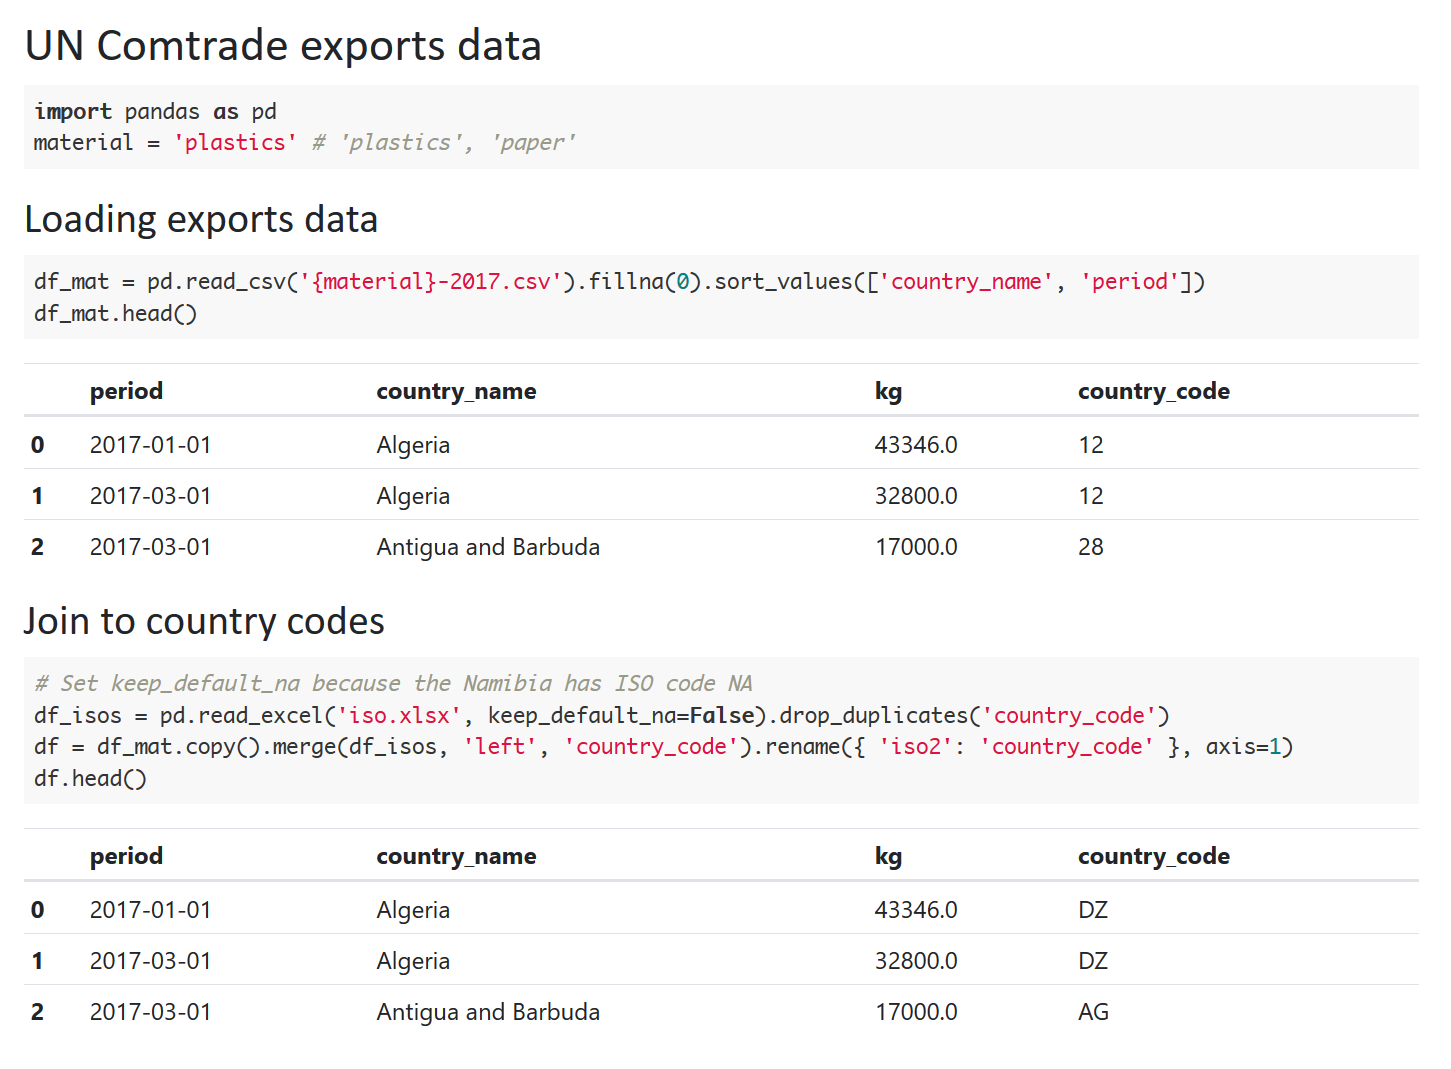
\includegraphics[scale=0.5]{notebook.png}
\caption{An excerpt from a Jupyter notebook by Financial Times reporters, which loads trade
  data from the UN trade database and adds ISO country codes.}
\label{fig:ft-uncomtrade}
\end{figure}

\section{Understanding how data scientists work}
\label{sec:background}

Data scientists often use general-purpose programming languages such as Python, but the kind of
code they write and the way they interact with the system is very different from how software
engineers work. This paper focuses on simple data wrangling and data exploration as done, for
example, by journalists analysing government datasets. This section illustrates how such data
analyses look and provides a justification for the design of our data exploration calculus.

% --------------------------------------------------------------------------------------------------

\subsection{Data wrangling in Jupyter}
\label{sec:background-jupyter}

Data analysts increasingly use notebook systems such as Jupyter or R Markdown, which
make it possible to combine text, equations and code with results of running the code such as tables
or visualizations. Notebooks blur the distinction between development and execution.
Data analysts write small snippets of code, run them to see results immediately and then revise
them.

% interactively based on the results. We aim to build foundations for such seamless integration
% of development and execution in a notebook environment.

Jupyter notebooks are used by a variety of users ranging from scientists who implement complex
models to journalists who load data, perform simple aggregations and create visualizations. Our
initial focus is on simple use cases, such as those of journalists. Tooling that makes notebook
systems more interactive and spreadsheet-like in such cases is of crucial importance as it enables
more people to produce reproducible and transparent data analyses.

As an example, consider the anlysis done by the Financial Times for an article on plastic
waste. The analysis joins datasets from Eurostat, UN Comtrade and more, aggregates the data and
builds a visualization comparing plastic waste flows in 2017 and 2018.
Figure~\ref{fig:ft-uncomtrade} shows an extract from one notebook from the data analysis.
The code of the analysis has a number of remarkable properties:
%
\begin{itemize}
\item There is no abstraction. The full analysis uses lambda functions as arguments to library calls,
  but it does not define any top-level functions. Parameterization is done by defining a list of
  inputs and then having a for loop, or by defining a top-level variable and setting its value.
  In our example, \ident{material} is set to \str{plastics} and a comment lists other options.
  This lets the analyst easily see and check the results of intermediate steps of the analysis.

\vspace{0.5em}
\item The code is structured as a sequence of commands. Some commands define a variable, either by
  loading data, or by transforming data loaded previously. Even in Python, data is often treated
  as immutable. Other commands produce an output that is displayed in the notebook.

\vspace{0.5em}
\item There are many corner cases, such as the fact that the \ident{keep\_default\_na} parameter
  needs to be set to handle Namibia correctly. These are discovered interactively by writing and
  running a code snippet and examining the output, so providing a rapid feedback is essential.
\end{itemize}

Many Jupyter notebooks are more complex than the example discussed here. They might define
helper functions or even structure code using object-oriented programming. However, simple
data analyses such as the one discussed here are frequent enough to pose an interesting and
important domain for programming tools research.

% --------------------------------------------------------------------------------------------------

\begin{figure}[b]
  \centering
  \subcaptionbox{
    \raggedright\footnotesize The Gamma script to aggregate Olympic medals. We select Rio 2016 games and
    count the number of distinct events per athlete. We then type `.' to choose
    further aggregation operations.
    \label{fig:gamma-dot}
  }{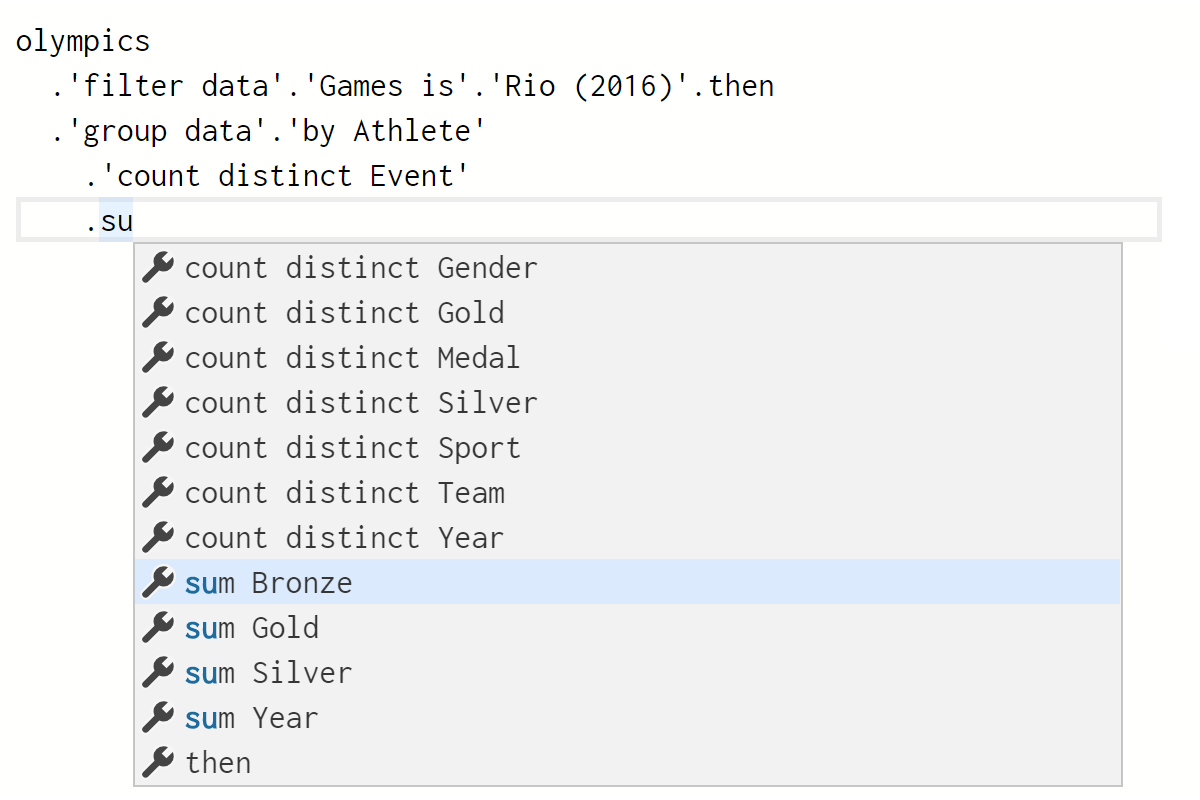
\includegraphics[scale=0.26]{gamma1.png}}
  \subcaptionbox{
    \raggedright\footnotesize Live preview in The Gamma programming environment. The table is produced as
      the data anlyst types and updates on-the-fly to show result at the current cursor position.
    \label{fig:gamma-preview}
  }{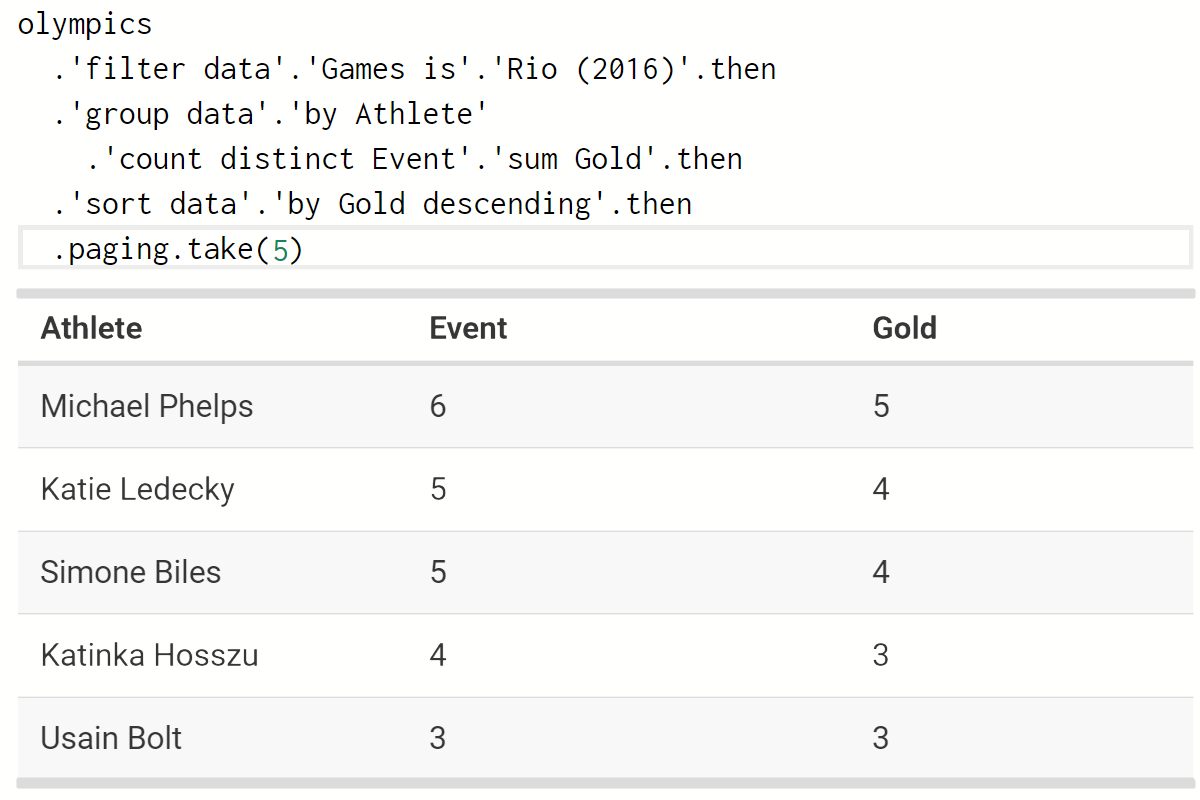
\includegraphics[scale=0.26]{gamma2.png}}
  \caption{\small TBD}
  \label{first-figure-with-subfigures}
\end{figure}

\subsection{Dot-driven data exploration in The Gamma}
\label{sec:background-gamma}

Data exploration of the kind discussed in the previous section has been the motivation
for a recent programming environment called The Gamma. The scripting language in The Gamma
captures the structure discussed above.

A script is a sequence of commands that can either define a
variable or produce an output. The language does not support top-level function declarations,
although we propose an extension that provides a simple abstraction mechanism and is compatible with
providing live previews in Section~X. Lambda functions can be used only as method
arguments.

Given the limited expressiveness of The Gamma, libraries for it are implemented in other languages, such as
JavaScript. More importantly, The Gamma supports type providers, which can be used to generate types,
on the fly, for accessing and exploring external data sources. Type providers provide object types
with members and The Gamma makes using those convenient by providing auto-complete when the user
types the dot symbol (`.') to access a member.

The combination of type providers and auto-complete on~``.'' makes it possible to complete a
large number of data exploration tasks through a very simple interaction of selecting operations from
a list. An example in Figure~\ref{fig:gamma-dot} summarizes data on Olympic medals using a type provider.
The names of identifiers such as \qident{sum Bronze} do not have
any special meaning -- they are merely members generated by the type provider, based on information
about the data source. The type provider used in this example generates an object with members for
different data transformations, such as \qident{group data}, which return furhter objects with
members for specifying transformation parameters, such as selecting the grouping key using
\qident{by Athlete}.

The Gamma is more complex than shown here -- it supports methods that can take
functions as arguments -- but the above example illustrates the fact that non-trivial data
exploration can be done using a very simple language.

We complement our theoretical work on foundations of live programming environments for data
exploration with an implementation for The Gamma. As discussed in the previous
section, the assumptions about structure of code that are explicit in The Gamma are also
implicitly present in Python and R data analyses produced by journalists, economists and
other users with other than  programming background. Consequently, our theoretical work
applies to simple data analyses using Python and readers not familiar with The Gamma
can assume that we use a small subset of Python.

% ==================================================================================================

% https://www.ft.com/content/360e2524-d71a-11e8-a854-33d6f82e62f8
% https://github.com/ft-interactive/recycling-is-broken-notebooks

\section{Live coding for data exploration}

% TODO: What is live coding? (Show preview while typing!)


This paper presents the foundations of a live coding environment for data exploration that
follows the analysis in the previous section. We consider simple data exploration tasks, such as
those done by journalists and we implement our ideas in the editor for TheGamma.

Figure~\ref{fig:gamma-preview} shows a TheGamma script exporing Olympic medal statistics in
our live coding environment. Before discussing the technical details, it is worth highlighting
a number of important points about our approach.

\begin{itemize}
\item\textbf{Real-world use cases.}
Our work has been motivated by the needs outlined in the previous section. In particular, we
have been focusing on a langauge that is simple, yet sufficient for completing basic data
exploration tasks that a journalist might want to do. We have used our live coding environment
to perform a number of simple data analyses looking at topics such as public government spending,
crises in financial markets and activities of a research institute. Qualitative observations about
our experience are reported in Section~X. Our tools can be used in any modern web browser and are
available as an open-source package.

\item\textbf{Text editor integration.}
Our approach is based on an ordinary text editor that allows unrestricted modification of the
code. Our parser supports error-recovery and we attempt to give previews whenever the code can be
correctly parsed and type-checked up to the current location. Notably, we do not, in general, know
how the user modified the code. This is in contrast with approaches based on structured editing
where the editor tracks what changes to code have been made. Using an ordinary text editor makes
providing live previews harder, but we believe that many users still favor the flexibility of
plain text editors.

\item\textbf{Data stay, code changes.}
Our focus has been on the scenario when input data is a static file that does not change, but the
data analyst modifies the source code. This is in contrast with work on incremental computation,
which focuses on scenarios where code stays the same, but input data change.

That said, many of the methods that we used for evaluating live previews such as maintaining
the dependency graph with nodes for individual syntactic elements are closely related to methods
used in incremental computation research. We do not attempt to combine the two, but note that
this is an interesting future direction.
\end{itemize}

\newpage
\begin{figure}
\raggedright
{\small\sffamily Programs, commands, terms, expressions and values}
\begin{equation*}
\hspace{-2em}
\begin{array}{lcl}
p &\narrow{=}& c_1; \ldots; c_n\\
c &\narrow{=}& \kvd{let}~x = t \lsep t\\
\end{array}
\qquad
\begin{array}{lcl}
t &\narrow{=}& o \lsep x \\
  &\narrow{|}& t.m(e, \ldots, e)
\end{array}
\qquad
\begin{array}{lcl}
e &\narrow{=}& t \lsep \lambda x\rightarrow e\\
v &\narrow{=}& o \lsep \lambda x\rightarrow e\\
\end{array}
\end{equation*}

\vspace{0.5em}
{\small\sffamily Evaluation contexts of expressions}
\begin{equation*}
\hspace{-2em}
\begin{array}{lcl}
C_e[-] &=& C_e[-].m(e_1, \ldots, e_n) ~\lsep~ o.m(v_1, \ldots, v_{m}, C_e[-], e_1,\ldots , e_n) ~\lsep~ -\\
C_c[-] &=& \kvd{let}~x = C_e[-] ~\lsep~ C_e[-]\\
C_p[-] &=& o_1;\; \ldots;\; o_{k};\; C_c[-];\; c_{1};\; \ldots;\; c_n\\
\end{array}
\end{equation*}

\vspace{0.5em}
{\small\sffamily Let elimination and member reduction}
\begin{equation*}
\hspace{-2em}
\begin{array}{ll}
\hspace{-0.5em}\begin{array}{l}
o_1;\; \ldots;\; o_{k};\; \kvd{let}~x=o;\; c_{1};\; \ldots; c_n \rightsquigarrow\\
\qquad  o_1;\; \ldots;\; o_{k};\; o; c_{1}[x\leftarrow o];\; \ldots; c_n[x\leftarrow o]\end{array} &
\quad\text{\rname{let}}\\[1.2em]
{o.m(v_1, \ldots, v_n) \rightsquigarrow_\epsilon o'}\implies
  {C_p[o.m(v_1, \ldots, v_n)] \rightsquigarrow C_p[o']} &
\quad\text{\rname{external}}
\end{array}
\end{equation*}

\vspace{-0.5em}
\caption{Syntax, contexts and reduction rules of the data exploration calculus}
\label{fig:dec-calculus}
\end{figure}

\section{Data exploration calculus}
\label{sec:calculus}

The \emph{data exploration calculus} is a small, formally tractable language for data exploration.
The calculus is not Turing-complete and it can only be used together with external libraries that
define what objects are available and what the behaviour of their members is. However, this is
sufficient to capture the simple data analyses discussed in Section~\ref{sec:background}. We
define the caluclus in this section and then use it as the basis for discussing our live preview
mechanism in Section~\ref{sec:formal}.

\subsection{Language syntax}
The calculus combines object-oriented features such as member access with functional features
such as lambda functions. The syntax is defined in Figure~\ref{fig:dec-calculus}. Object values
$o$ are defined by external libraries that are used in conjunction with the core calculus.

A program $p$ in the data exploration calculus consists of a sequence of commands $c$. A command
can be either let binding or a term. Let bindings define variables $x$ that can be used in
subsequent commands. The calculus supports lambda functions, but they
can only appear as arguments in method calls. A term $t$ can be a value, variable or a
member access, while an expression $e$, which can appear as an argument in member access,
can be a lambda function or a term.\footnote{Similar but weaker restrictions on the use of lambda functions
exist in other languages. To guide type inference, lambda functions in C\# can appear as either
method arguments or assigned to an explicitly typed variable.}

\subsection{Operational semantics}
\label{sec:calculus-semantics}

The data exploration calculus is a call-by-value language. We model the evaluation as a small-step
reduction $\rightsquigarrow$. Fully evaluating a program results in an irreducible sequence of
objects $o_1;\; \ldots;\; o_n$ which can be displayed as intermediate results of the data analysis. The
operational semantics is parameterized by a relation $\rightsquigarrow_\epsilon$ that models
the functionality of the external libraries used with the calculus and defines reduction rules
for member accesses. The relation has the following form:
%
\begin{equation*}
o_1.m(v_1, \ldots, v_n) \rightsquigarrow_\epsilon o_2
\end{equation*}
%
Figure~\ref{fig:dec-calculus} defines the reduction rules in terms of $\rightsquigarrow_\epsilon$
and evaluation contexts; $C_e$ specifies left-to-right evaluation of arguments of a method call,
$C_c$ specifies evluation of a command and $C_p$ defines top-to-bottom evaluation of a program.
The rule \rname{external} applies reductions provided by an external library in a
call-by-value order and \rname{let} substitutes a value of an evaluated variable in
all subsequent commands. Note that \rname{let} leaves the value of the variable
in the resulting list of commands.

\subsection{Properties}

DEFINE $\rightsquigarrow^{*}$ as a reflexive, transitive closure of $\rightsquigarrow$

DEFINE $\rightsquigarrow_\ident{let}$ (on a program) - CBN subsitution

\begin{definition}[External library]
\label{def:external}

Satsifies \emph{compositionality} such that:

Given $e_0, e_1, \ldots, e_n$ and $e'_0, e'_1, \ldots, e'_n$ and $m$ such that
$e_0.m(e_1, \ldots, e_n) \rightsquigarrow^{*} o$ and
$e'_0.m(e'_1, \ldots, e'_n) \rightsquigarrow^{*} o'$ then
if for any contexts
$C_0, C_1, \ldots, C_n$ it holds that if $C_i[e_i] \rightsquigarrow^{*} o_i$ and $C_i[e'_i] \rightsquigarrow^{*} o_i$ for some $o_i$
then $o = o'$.
\end{definition}

TBD: LET above should leave the evaluated object in the list of commmands

LET ELIMINATION DOES NOT CHANGE RESULTS

Let elimination $\rightsquigarrow_\ident{let}$ such that, using  capture-avoiding substitution,
$C[\kvd{let}~x=e_1~\kvd{in}~e_2] \rightsquigarrow_\ident{let} C[e_2[x\leftarrow e_1]]$

Let elimination does not affect the result, i.e.~if $e \rightsquigarrow_{\ident{let}} e'$
and $e'\rightsquigarrow_\beta e''$ then also $e\rightsquigarrow_\beta e''$

\begin{lem}[Let elimination for a program]
\label{thm:let-lang-elimination}
does not matter
\end{lem}

\newpage

% ==================================================================================================

\section{Formalising live coding environment}
\label{sec:formal}

A naive way of providing live previews during code editing would be to re-evaluate the code
after each change. This would be wasteful -- for example, when writing
code, most changes are additive and the preview can be updated by evaluating just the newly added
code. In this section, we develop foundations for an efficient way of displaying live previews
for the data exploration calculus.

% --------------------------------------------------------------------------------------------------

\subsection{Maintaining dependency graph}
\label{sec:formal-deps}

The key idea behind our method is to maintain a dependency graph \cite{dependencies} with
nodes representing individual operations of the computation that can be (partially) evaluated
to obtain a preview. Each time the program text is modified, we parse it afresh (using an
error-recovering parser) and bind the abstract syntax tree to the dependency graph.
When binding a new expression to the graph, we reuse previously created nodes as long as
they have the same dependencies. For expressions that have a new structure, we create new nodes.

The nodes of the graph serve as unique keys into a lookup table with previously
evaluated parts of the program. When a preview is requested for an expression, we use the graph
node bound to the expression to find a preview. If a preview has not been evaluated, we force
the evaluation of all dependencies in the graph and then evaluate the operation represented by
the current node.

% --------------------------------------------------------------------------------------------------

\begin{figure}[b]
\centering
\subcaptionbox{
  \raggedright\small
  Graph constructed from the following initial expression:
  $\kvd{let}~x = \num{15}~\kvd{in}~\ident{data.skip}(\num{10}).\ident{take}(x)$
  \label{fig:dep-graph-a}
}{
  $\xymatrix{
  \bnd{val}(\num{10}) & \bnd{val}(\num{15})\\
  \bnd{mem}(\ident{skip},s_0)\ar[d]_{\blbl{arg}(0)} \ar[u]^{\blbl{arg}(1)} &
  \bnd{mem}(\ident{take},s_1)\ar[l]_{\blbl{arg}(0)} \ar[u]_{\blbl{arg}(1)}\\
  \bnd{var}(\ident{data})
  }\qquad$
}
\hspace{1em}
\subcaptionbox{
  \raggedright\small
  Updated graph after changing $x$ to $10$:
  $\kvd{let}~x = \num{10}~\kvd{in}~\ident{data.skip}(\num{10}).\ident{take}(x)$
  \label{fig:dep-graph-b}
}{
  $\xymatrix{
  \bnd{val}(\num{10})&\\
  \bnd{mem}(\ident{skip}, s_0)\ar[d]_{\blbl{arg}(0)} \ar[u]^{\blbl{arg}(1)} &
  \bnd{mem}(\ident{take}, s_2)\ar[l]_{\blbl{arg}(0)} \ar@/_/[lu]_{\blbl{arg}(1)}\\
  \bnd{var}(\ident{data})
}\qquad$
}
\caption{Dependency graphs formed by two steps of the live programming process. }
\label{fig:dep-graph}
\end{figure}

% --------------------------------------------------------------------------------------------------

\subsubsection{Elements of the graph}
The nodes of the graph represent individual operations of the computation. In our design, the nodes
are used as cache keys, so we attach a unique symbol $s$ to some of the nodes. That way, we can
create two unique nodes representing, for example, access to a member named \ident{take} which
differ in their dependencies.

Furthermore, the graph edges are labeled with labels indicating the kind of dependency. For
a method call, the labels are ``first argument'', ``second argument'' and so on. Writing
$s$ for symbols and $i$ for integers, nodes (vertices) $\bndclr{v}$ and edge labels $\blblclr{l}$
are defined as:
%
\begin{equation*}
\begin{array}{rcll}
\bndclr{v}&=&\bnd{val}(o) \lsep \bnd{var}(x)\lsep \bnd{mem}(m, s)\lsep \bnd{fun}(x, s)&(\textit{Vertices})\\
\blblclr{l}&=&\blbl{body} \lsep \blbl{arg}(i)&(\textit{Edge labels})\\
\end{array}
\end{equation*}
%
The \bnd{val} node represents a primitive value and contains the object itself. Two occurrences
of $\num{10}$ in the source code will be represented by the same node. Member access \bnd{mem}
contains the member name, together with a unique symbol $s$ -- two member access nodes with
different dependencies will contain a different symbol. Dependencies of member access are labeled
with \blbl{arg} indicating the index of the argument (the instance has index $0$ and arguments
start with $1$). Finally, nodes \bnd{fun} and \bnd{var} represent function values and variables
bound by $\lambda$ abstraction. For simplicity, we use variable names rather than de Bruijn
indices and so renaming a bound variable forces recomputation.

% --------------------------------------------------------------------------------------------------

\subsubsection{Example graph}
Figure~\ref{fig:dep-graph} illustrates how we construct and update the
dependency graph. Node representing $\ident{take}(x)$ depends on the argument -- the
number $\num{15}$ -- and the instance, which is a node representing $\ident{skip}(\num{10})$.
This, in turn, depends on the instance \ident{data} and the number $\num{10}$. Note that variables
bound via \kvd{let} binding such as $x$ do not appear as $\bnd{var}$ nodes. The node using it
depends directly on the node representing the expression that is assigned to $x$.

After changing the value of $x$, we create a new graph. The dependencies of the node
$\bnd{mem}(\ident{skip}, s_0)$ are unchanged and so the symbol $s_0$ attached to the node remains
the same and previously computed previews can be reused. This part of the program is not recomputed.
The $\blbl{arg}(1)$ dependency of the \ident{take} call
changed and so we create a new node $\bnd{mem}(\ident{skip}, s_2)$ with a fresh symbol $s_2$.
The preview for this node is then computed as needed using the already known values of its
dependencies.

% --------------------------------------------------------------------------------------------------

\subsubsection{Reusing graph nodes}
The binding process takes an expression and constructs a dependency graph reusing existing nodes
when possible. For this, we use a lookup table of member access and function value nodes. The key
in the lookup table is formed by a node kind (for disambiguation) together with a list of
dependencies. A node kind is a member access containing the member name or a function containing
the bound variable name; a lookup table $\Delta$ then maps a node kind with a list of dependencies
to a cached node:
%
\begin{equation*}
\begin{array}{ll}
\bkndclr{k}~=~\bknd{fun}(x)~|~\bknd{mem}(m)&(\textit{Node kinds})\\[0.2em]
\Delta(\bkndclr{k}, [(\bndclr{v_1},\blblclr{l_1}), \ldots, (\bndclr{v_n},\blblclr{l_n})])  & (\textit{Lookup for a node})
\end{array}
\end{equation*}
%
The example on the second line looks for a node of a kind $\bkndclr{k}$ that has dependencies
$\bndclr{v_1}, \ldots, \bndclr{v_n}$ labeled with labels $\blblclr{l_1}, \ldots, \blblclr{l_n}$.
We write $\Delta(\bndclr{k}, l)\!\downarrow$ when a value for a given key is not defined.
For example, when creating the graph in Figure~\ref{fig:dep-graph-b},
we perform the following lookup for the \ident{skip} member access:
%
\[ \Delta(\bknd{mem}(\ident{skip}), [(\bnd{var}(\ident{data}),\blbl{arg}(0)), (\bnd{val}(\num{10}), \blbl{arg}(1))]) \]
%
The lookup returns the node $\bnd{mem}(\ident{skip}, s_0)$ known from the previous step. We then perform
the following lookup for the \ident{take} member access:
%
\[ \Delta(\bknd{mem}(\ident{take}), [(\bnd{mem}(\ident{skip}, s_0),\blbl{arg}(0)), (\bnd{val}(\num{10}), \blbl{arg}(1))]) \]
%
In the previous graph, the argument of \ident{take} was $\num{15}$ rather than $\num{10}$ and so
this lookup fails. We then construct a new node $\bnd{mem}(\ident{take}, s_2)$ using a fresh
symbol $s_2$.

% --------------------------------------------------------------------------------------------------

\begin{figure*}[t]
\begin{equation*}
\hspace{-3.5em}
\begin{array}{ll}
\ident{bind-expr}_{\Gamma, \Delta}(e_0.m(e_1, \ldots, e_n)) = \bndclr{v}, (\{\bndclr{v}\} \cup V_0 \cup \ldots \cup V_n, E \cup E_0 \cup \ldots \cup E_n) &(1)~~\\
\quad \textnormal{when}~\bndclr{v_i}, (V_i, E_i) = \ident{bind-expr}_{\Gamma, \Delta}(e_i)
~\textnormal{and}~\bndclr{v} = \Delta(\bknd{mem}(m),[(\bndclr{v_0}, \blbl{arg}(0)), \ldots, (\bndclr{v_n}, \blbl{arg}(n))])\\
\quad \textnormal{let}~E = \{ (\bndclr{v}, \bndclr{v_0}, \blbl{arg}(0)), \ldots, (\bndclr{v}, \bndclr{v_n}, \blbl{arg}(n))\}
\\[1em]
\ident{bind-expr}_{\Gamma, \Delta}(e_0.m(e_1, \ldots, e_n)) = \bndclr{v}, (\{\bndclr{v}\} \cup V_0 \cup \ldots \cup V_n, E \cup E_0 \cup \ldots \cup E_n)&(2)\\
\quad \textnormal{when}~\bndclr{v_i}, (V_i, E_i) = \ident{bind-expr}_{\Gamma, \Delta}(e_i)
~\textnormal{and}~\Delta(\bknd{mem}(m),[(\bndclr{v_0}, \blbl{arg}(0)), \ldots, (\bndclr{v_n}, \blbl{arg}(n))])\!\downarrow\\
\quad \textnormal{let}~\bndclr{v} = \bnd{mem}(m, s), s~\textnormal{fresh}
~\textnormal{and}~E = \{ (\bndclr{v}, \bndclr{v_0}, \blbl{arg}(0)), \ldots, (\bndclr{v},\bndclr{v_n}, \blbl{arg}(n)) \}
\\[1em]
\ident{bind-expr}_{\Gamma, \Delta}(\lambda x \rightarrow e) = \bndclr{v}, (\{\bndclr{v}\} \cup V, \{e\} \cup E)&(3)\\
\quad \textnormal{when}~\Gamma_1 = \Gamma \cup \{ x, \bnd{var}(x) \}
~\textnormal{and}~\bndclr{v_0}, (V, E) = \ident{bind-expr}_{\Gamma_1, \Delta}(e)
~\textnormal{and}~\bndclr{v} = \Delta(\bknd{fun}(x),[(\bndclr{v_0}, \blbl{body})])\\
\quad \textnormal{let}~e = (\bndclr{v}, \bndclr{v_0}, \blbl{body})
\\[1em]
\ident{bind-expr}_{\Gamma, \Delta}(\lambda x \rightarrow e) = \bndclr{v}, (\{\bndclr{v}\} \cup V, \{e\} \cup E)&(4)\\
\quad \textnormal{when}~\Gamma_1 = \Gamma \cup \{ x, \bnd{var}(x) \}
~\textnormal{and}~\bndclr{v_0}, (V, E) = \ident{bind-expr}_{\Gamma_1, \Delta}(e)
~\textnormal{and}~\Delta(\bknd{fun}(x),[(\bndclr{v_0}, \blbl{body})])\!\downarrow\\
\quad \textnormal{let}~\bndclr{v} = \bnd{fun}(x, s), s~\textnormal{fresh}
~\textnormal{and}~e = (\bndclr{v},\bndclr{v_0},\blbl{body})
\\[1em]
\ident{bind-expr}_{\Gamma, \Delta}(o) = \bnd{val}(o), (\{ \bnd{val}(o) \}, \emptyset) &(5)
\\[1em]
\ident{bind-expr}_{\Gamma, \Delta}(x) = \bndclr{v}, (\{ \bndclr{v} \}, \emptyset)~\textnormal{when}~\bndclr{v} = \Gamma(x)&(6)
\end{array}
\end{equation*}
\caption{Binding rules that define a construction of a dependency graph for an expression.}
\label{fig:binding-rules-expr}
\end{figure*}

% --------------------------------------------------------------------------------------------------

\begin{figure*}[t]
\begin{equation*}
\hspace{-3.5em}
\begin{array}{ll}
\ident{bind-prog}_{\Gamma, \Delta}(\kvd{let}~x=e; c_2; \ldots; c_n) = \bndclr{v_1};\ldots;\bndclr{v_n}, (\{\bndclr{v_1}\} \cup V \cup V_1, E \cup E_1)
  \hspace{9.35em}&(7)\\
\quad \textnormal{let}~\bndclr{v_1}, (V_1,E_1) = \ident{bind-expr}_{\Gamma,\Delta}(e_1)~\textnormal{and}~\Gamma_1 = \Gamma \cup \{(x,\bndclr{v_1})\} \\
\quad \textnormal{and}~\bndclr{v_2}; \ldots; \bndclr{v_n}, (V, E) = \ident{bind-prog}_{\Gamma_1, \Delta}(c_2; \ldots; c_n)
\\[1em]
\ident{bind-prog}_{\Gamma, \Delta}(e; c_2; \ldots; c_n) = \bndclr{v_1};\ldots;\bndclr{v_n}, (\{\bndclr{v_1}\} \cup V \cup V_1, E \cup E_1)&(8)\\
\quad \textnormal{let}~\bndclr{v_1}, (V_1,E_1) = \ident{bind-expr}_{\Gamma,\Delta}(e)
~\textnormal{and}~\bndclr{v_2}; \ldots; \bndclr{v_n}, (V, E) = \ident{bind-prog}_{\Gamma_1, \Delta}(c_2; \ldots; c_n)
\\[1em]
\ident{bind-prog}_{\Gamma, \Delta}([]) = [], (\emptyset, \emptyset)&(9)
\end{array}
\end{equation*}
\caption{Binding rules that define a construction of a dependency graph for a program.}
\label{fig:binding-rules-prog}
\end{figure*}


% --------------------------------------------------------------------------------------------------

\subsection{Binding expressions to a graph}
\label{sec:formal-bind}

After parsing updated code, we update the dependency graph and link each node of the abstract
syntax tree to a node of the dependency graph. This process is called
binding and is defined by the \ident{bind-expr} function (Figure~\ref{fig:binding-rules-expr})
and \ident{bind-prog} function (Figure~\ref{fig:binding-rules-prog}). Both functions are
annotated with a lookup table $\Delta$ discussed in Section~\ref{sec:formal-deps} and a variable
context $\Gamma$. The variable context is a map from variable names to dependency graph nodes and
is used for variables bound using \kvd{let} binding.

When applied on an expression $e$, binding $\ident{bind-expr}_{\Gamma,\Delta}(e)$ returns
a node $\bndclr{v}$ corresponding to the expression $e$ paired with a dependency graph $(V, E)$.
In the graph, $V$ is a set of nodes $\bndclr{v}$ and $E$ is a set of labeled edges
$(\bndclr{v_1}, \bndclr{v_2}, \blblclr{l})$. We attach the label directly to the edge rather than
keeping a separate colouring function as this makes the formalisation simpler.
The $\ident{bind-prog}_{\Gamma,\Delta}$ function works similarly, but takes a sequence of
commands and returns a sequence of nodes.

\subsubsection{Binding expressions.} When binding member access, we use \ident{bind-expr} recursively
to get a node and a dependency graph for each sub-expression. The nodes representing sub-expressions are
then used as dependencies for lookup into $\Delta$, together with their labels. If a node already
exists in $\Delta$ it is reused (1). Alternativelym, we create a new node containing a fresh symbol~(2).

If a lambda function uses its argument, we will not be able to evaluate its body. In this case, the
graph node bound to a function will depend on a synthetic node $\bnd{var}(x)$ that represents the
variable with unknown value. When binding a function, we create the synthetic variable and add it
to the variable context $\Gamma_1$ before binding the body. As with member access, the node
representing a function may (3) or may not (4) be already present in the lookup table.

\subsubsection{Binding programs.} When binding a program, we bind the first command and then
recursively process remaining commands until we reach an empty list of commands (9).
For \kvd{let} binding (7), we bind the expression $e$ assigned to the variable to obtain a
graph node $\bndclr{v_1}$. We then bind the remaining commands using a variable context $\Gamma_1$
that maps the value of the variable to the graph node $\bndclr{v_1}$. The variable context is used
when binding a variable (6) and so all variables declared using \kvd{let} binding will be bound to
a graph node representing the value assigned to the variable. When the command is just an
expression (8), we bind the expression using \ident{bind-expr}.

% --------------------------------------------------------------------------------------------------

\begin{figure}
\begin{equation*}
\begin{array}{l}
\ident{update}_{V,E}(\Delta_{i-1}) = \Delta_i~\textnormal{such that:}
\\[0.75em]
\quad\Delta_{i}(\bknd{mem}(m), [(\bndclr{v_0},\blbl{arg}(0)),\ldots, (\bndclr{v_n},\blbl{arg}(n))]) = \bnd{mem}(m, s)\\
\quad\quad \textnormal{when}~\bnd{mem}(m, s) \in V
~\textnormal{and}~(\bnd{mem}(m, s), \bndclr{v_i}, \blbl{arg}(i)) \in E~\textnormal{for}~i\in 0,..,n
\\[0.75em]
\quad\Delta_{i}(\bknd{fun}(x), [(\bndclr{v_1},\blbl{body})]) = \bnd{fun}(x, s)\\
\quad\quad \textnormal{when}~\bnd{fun}(x, s) \in V
~\textnormal{and}~(\bnd{fun}(x, s), \bndclr{v_1}, \blbl{body}) \in E
\\[0.75em]
\quad\Delta_{i}(\bkndclr{v}) = \Delta_{i-1}(\bkndclr{v})\quad \textnormal{(otherwise)}
\end{array}
\end{equation*}
\vspace{-1em}
\caption{Updating the node cache after binding a new graph}
\label{fig:loop}
\vspace{-0.5em}
\end{figure}

% --------------------------------------------------------------------------------------------------

\subsection{Edit and rebind loop}

The binding process formalised in Section~\ref{sec:formal-bind} specifies how to update the
dependency graph after updated program text is parsed. During live coding, this is done
repeatedly as the programmer edits code. Throughout the process, we maintain a series of
lookup table states $\Delta_0, \Delta_1, \Delta_2, \ldots$ The initial lookup table is
empty, i.e.~$\Delta_0 = \emptyset$. At a step $i$, we parse a program $p_i$ (consisting of
several commands) and obtain a new dependency graph using the previous $\Delta$. The result is
a sequence of nodes corresponding to commands of the program and a graph $(V, E)$:
%
\begin{equation*}
\bndclr{v_1}; \ldots; \bndclr{v_n}, (V, E) = \ident{bind-prog}_{\emptyset, \Delta_{i-1}}(p_i)
\end{equation*}
%
The new state of the cache is computed by calling the $\ident{update}_{V, E}(\Delta_{i-1})$ function
defined in Figure~\ref{fig:loop}. The function adds newly created nodes from the graph
$(V, E)$ to the previous cache $\Delta_{i-1}$ and returns a new cache $\Delta_{i}$. We only cache
nodes for function and member accesses -- nodes for variables and primitive values will remain
the same thanks to the way they are constructed.

% ==================================================================================================

\section{Evaluating previews}
\label{sec:previews}

The binding process described in the previous section constructs a dependency graph after code
changes. The nodes in the dependency graph correspond to individual operations that will be performed
when running the program. When evaluating a preview, we attach (partial) results to
nodes of the graph. Since the binding process reuses nodes when their dependencies do not change,
previews for expressions (or sub-expressions) of a program can be reused when updating a preview.

In this section, we describe how previews are evaluated. The evaluation is done over the dependency
graph, rather than over the structure of the program expressions as in the operational semantics
given in Section~\ref{sec:calculus-semantics}. We analyse the preview evaluation formally in
Section~\ref{sec:properties} and show that the resulting previews are the same as the result we
would get by directly evaluating the code and, also, that no recomputation occurs when code is
edited in certain ways.

% --------------------------------------------------------------------------------------------------

\subsection{Previews and delayed previews}

Programs in the data exploration calculus consist of sequence of commands. Those can always be
evaluated to a value with a preview that can be displayed to the user. However, we also support
previews for all sub-expressions. This can be problematic if the current sub-expression is inside
the body of a function. For example:
%
\begin{equation*}
\begin{array}{l}
\kvd{let}~\ident{top} = \ident{movies}.\ident{take}(\num{10}).\ident{map}(\lambda x \rightarrow x.\ident{getReleased}().\ident{format}(\str{dd-mm-yyyy}))
\end{array}
\end{equation*}
%
Here, we can directly evaluate sub-expressions \ident{movies} and $\ident{movies}.\ident{take}(\num{10})$,
but not $x.\ident{getReleased}()$ and $x.\ident{getReleased}().\ident{format}(\str{dd-mm-yyyy})$
because they contain a free variable $x$. Our preview evaluation algorithm addresses this by
producing two kinds of previews. A \emph{fully evaluated preview} is just a value, while
a \emph{delayed preview} is a partially evalauted expression with free variables:

\begin{equation*}
\begin{array}{rcll}
p&=&o \lsep  \lambda x\rightarrow e&\quad(\textit{Fully evaluated previews})\\
d&=&p \lsep  \llbracket e \rrbracket_\Gamma&\quad(\textit{Evaluated and delayed previews})\\
\end{array}
\end{equation*}
%
A fully evaluated preview $p$ can be either a primitive object or a function value with no free
variables. A possibly delayed preview $d$ can be either an evaluated preview $p$ or an expression
$e$ that requires variables $\Gamma$. For simplicity, we use an untyped language and so $\Gamma$
is just a list of variables $x_1, \ldots, x_n$.

A delayed preview is not necessarily the body of a lambda function as it appears in the source
code. We partially evaluate sub-expressions of the body that do not have free variables or that
have free variables bound by an earlier let binding.

Our implementation does not currently display
delayed previews to the user, but there is a number of possible approaches for doing that.
Most interestingly, since lambda functions always appear as arguments of a member access, we could
force the evaluation of the surrounding expression, capture (a number of) values passed as inputs
to the lambda function and display a preview based on those. Finally, in Section~\ref{sec:design},
we also consider a more speculative design for an abstraction mechanism that supports live previews
that could, in some cases, replace lambda function.

% --------------------------------------------------------------------------------------------------

\begin{figure*}[b]
\begin{equation*}
\hspace{-2.5em}
\begin{array}{l}
\inference[\rname{lift-expr}~]
  {\bndclr{v} \Downarrow \llbracket e \rrbracket_\Gamma}
  {\bndclr{v} \Downarrow_{\ident{lift}} \llbracket e \rrbracket_\Gamma}
\\
\\
\inference[\rname{lift-prev}~]
  {\bndclr{v} \Downarrow p}
  {\bndclr{v} \Downarrow_{\ident{lift}} \llbracket p \rrbracket_\emptyset}
\\
\\
\inference[\rname{val}~]
  {~}
  {\bnd{val}(o) \Downarrow o }
\\
\\
\inference[\rname{var}~]
  {~}
  {\bnd{var}(x) \Downarrow \llbracket x \rrbracket_x}
  \\[0.5em]~
\end{array}
\qquad\quad
\begin{array}{l}
\inference[\rname{fun-val}~]
  { (\bnd{fun}(x, s), \bndclr{v}, \blbl{body}) \in E & \bndclr{v} \Downarrow p }
  { \bnd{fun}(x, s) \Downarrow \lambda x\rightarrow p }
\\
\\
\inference[\rname{fun-bind}~]
  { (\bnd{fun}(x, s), \bndclr{v}, \blbl{body}) \in E & \bndclr{v} \Downarrow \llbracket e \rrbracket_{x} }
  { \bnd{fun}(x, s) \Downarrow \lambda x\rightarrow e }
\\
\\
\inference[\rname{fun-expr}~]
  { (\bnd{fun}(x, s), \bndclr{v}, \blbl{body}) \in E & \bndclr{v} \Downarrow \llbracket e \rrbracket_{x,\Gamma} }
  { \bnd{fun}(x, s) \Downarrow \llbracket \lambda x\rightarrow e \rrbracket_\Gamma }
\\[0.5em]~
\end{array}
\end{equation*}
\begin{equation*}
\hspace{-2.5em}
\begin{array}{l}
\inference[\rname{mem-val}~]
  { \forall i\in\{0\ldots k\}.(\bnd{mem}(m, s), \bndclr{v_i}, \blbl{arg}(i)) \in E & \bndclr{v_i} \Downarrow p_i
    & p_0.m(p_1, \ldots, p_k) \rightsquigarrow_\epsilon p }
  { \bnd{mem}(m, s) \Downarrow p }
\\
\\
\inference[\rname{mem-expr}~]
  { \forall i\in\{0\ldots k\}.(\bnd{mem}(m, s), \bndclr{v_i}, \blbl{arg}(i)) \in E & \exists j\in\{0\ldots k\}.\bndclr{v_j}\diagup\hspace{-1em}\Downarrow p_j
   & \bndclr{v_i} \Downarrow_{\ident{lift}} \llbracket e_i \rrbracket_{\Gamma_i}  }
  { \bnd{mem}(m, s) \Downarrow \llbracket e_0.m(e_1, \ldots, e_k) \rrbracket_{\Gamma_0,\ldots,\Gamma k} }
\\
\end{array}
\end{equation*}

\caption{Rules that define evaluation of previews over a dependency graph for a program}
\label{fig:eval}
\end{figure*}

% --------------------------------------------------------------------------------------------------

\subsection{Evaluation of previews}
The evaluation of previews is defined in Figure~\ref{fig:eval}. Given a dependency graph $(V, E)$,
we define a relation $\bndclr{v}\Downarrow d$ that evaluates a sub-expression corresponding to
the node $\bndclr{v}$ to a possibly delayed preview $d$. The nodes $V$ and edges $E$ of the
dependency graph are parameters of the $\Downarrow$ relation, but they do not change during the
evaluation and so we do not explicity write them.

The auxiliary relation $\bndclr{v}\Downarrow_{\ident{lift}} d$ always evaluates
to a delayed preview. If the ordinary evaluation returns a delayed preview, so does the auxiliary
relation \rname{lift-expr}. If the ordinary evaluation returns a value, the value is wrapped
into a delayed preview requiring no variables \rname{lift-prev}.
%
A node representing a value is evaluated to a value \rname{val} and a node representing
an unbound variable is reduced to a delayed preview that requires the variable and returns its
value~\rname{var}.

For member access, we distinguish two cases. If all arguments evaluate to values \rname{member-val},
then we use the evaluation relation defined by external libraries $\rightsquigarrow_\epsilon$ to
immediately evaluate the member access and produce a value. If some of the arguments are
delayed \rname{member-expr}, because the member access is inside the body of a lambda function,
we produce a delayed member access expression that requires the union of the variables
required by the individual arguments.

The evaluation of function values is similar, but requires three cases. If the body can
be reduced to a value with no unbound variables \rname{fun-val}, we return a lambda function that
returns the value. If the body requires only the bound variable \rname{fun-bind}, we return a
lambda function with the delayed preview as the body. If the body requires further variables,
the result is a delayed preview.

\subsection{Caching of evaluated previews}
\label{sec:previews-cache}

For simplicity, the relation $\Downarrow$ in Figure~\ref{fig:eval} does not specify how previews
are cached and linked to graph nodes. In practice, this is done by maintaining a lookup table
from graph nodes $\bndclr{v}$ to (possibly delayed) previews $p$.
Whenever $\Downarrow$ is used to obtain a preview for a graph node, we first
attempt to find an already evaluated preview using the lookup table. If the preview has not
been previously evaluated, we evaluate it and add it to the lookup table.

The cached evaluated previews can be reused in two ways. First, multiple nodes can
depend on one sub-graph in a single dependency graph (if the same sub-expression appears
twice in the program). Second, the keys of the lookup table are graph nodes and nodes are
reused when a new dependency graph is constructed after the user edits the source code.

\subsection{Theories of delayed previews}
The operational semantics presented in this paper serves two purposes. It gives a simple guide
for implementing text-based live coding environments for data science and we use it to prove that
our optimized way of producing live previews is correct. However, some aspects of our mechanism
are related to important work in semantics of programming languages and deserve to be mentioned.

The construction of delayed previews is related to meta-programming. Assuming
we have delayed previews $\llbracket e_0 \rrbracket_x$ and $\llbracket e_1 \rrbracket_y$ and
we invoke a member $m$ on $e_0$ using $e_1$ as an argument. To do this, we construct a new
delayed preview $\llbracket e_0.m(e_1) \rrbracket_{x, y}$. This operation is akin to expression
splicing from meta-programming \cite{metaml,quotations}.

The semantics of delayed previews can be more formally captured by Contextual Modal Type Theory
(CMTT) \cite{cmtt} and comonads \cite{cmtt-denotation}. In CMTT, $\lbrack \Psi \rbrack A$ denotes
that a proposition $A$ is valid in context $\Psi$, which is similar to our delayed previews written
as $\llbracket A \rrbracket_\Psi$. CMTT defines rules for composing context-dependent propositions
that would allow us to express the splicing operation used in \rname{mem-expr}. In categorical
terms, the context-dependent proposition can be modeled as an indexed comonad \cite{effectrev,graded}.
The evaluation of a preview with no context dependencies (built implicitly into our evaluation rules)
corresponds to the counit operation of a comonad and would be explicitly written as
$\llbracket A \rrbracket_\emptyset \rightarrow A$.

% ==================================================================================================

\section{Properties of live coding environment}
\label{sec:properties}

The use of a dependency graph when evaluating previews makes it possible to cache partial results
through a mechanism discussed in Section~\ref{sec:formal-deps} and Section~\ref{sec:previews-cache}.
The mechanism satisfies two properties. First, if we evaluate a preview using dependency
graph with caching, it is the same as the value we would obtain by evaluating the expression
directly. Second, the evaluation of previews using dependency graphs reuses -- in some cases --
previously evaluated partial results. In other words, we show that the mechanism is correct
and implements a useful optimization.

% --------------------------------------------------------------------------------------------------

\subsection{Correctness of previews}
\label{sec:properties-correct}

To show that the evaluated previews are correct, we prove two properties. Correctness
(Theorem~\ref{thm:correcntess}) guarantees that, no matter how a dependency graph is constructed,
when we use it to evaluate previews for a program, the previews are the same as the values we
would obtain by evaluating the program commands directly. Determinacy (Theorem~\ref{thm:determinacy})
guarantees that if we cache a preview for a graph node and update the graph, the preview we would
evaluate using the updated graph would be the same as the cached preview.

To simplify the proofs, we consider programs without let bindings. This is possible, because
eliminating let bindings does not change the result of evaluation, as shown earlier in
Lemma~\ref{thm:let-lang-elimination}, and it also does not change the constructed dependency graph
as shown below in Lemma~\ref{thm:let-grp-elimination}.

\begin{lem}[Let elimintion for a dependency graph]
\label{thm:let-grp-elimination}
Given programs $p_1, p_2$ such that $p_1 \rightsquigarrow_\ident{let} p_2$ and a lookup table
$\Delta_0$ then if $\bndclr{v_1}; \ldots; \bndclr{v_n}, (V, E) = \ident{bind-prog}_{\emptyset, \Delta_0}(p_1)$ and
$\bndclr{v'_1};\ldots;\bndclr{v'_n}, (V', E') = \ident{bind-prog}_{\emptyset, \Delta_1}(p_2)$ such that $\Delta_1 = \ident{update}_{V, E}(\Delta_0)$
then for all $i$, $\bndclr{v_i} = \bndclr{v'_i}$ and also $(V, E) = (V', E')$.
\end{lem}
\begin{proof}
Assume $p_1 = c_1; \ldots; c_{k-1}; \kvd{let}~x=e; c_{k+1};\ldots; c_n$ and the let binding is
eliminated resulting in $p_2 = c_1; \ldots; c_{k-1}; e; c_{k+1}[x\leftarrow e];\ldots; c_n[x\leftarrow e]$.
When binding $p_1$, the case $\ident{bind-prog}_{\Gamma,\Delta}(\kvd{let}~x=e)$ is handled using (7)
and the node resulting from binding $e$ is added to the graph $V, E$. It is then referenced each
time $x$ appears in subsequent commands $c_{k+1}; \ldots; c_n$.
When binding $p_2$, the node resulting from binding $e$ is a primitive value or a node already
present in $\Delta_1$ (added by $\ident{update}_{V, E}$) and is reused each time
$\ident{bind-expr}_{\Gamma,\Delta_1}(e)$ is called.
\end{proof}

The Lemma~\ref{thm:let-grp-elimination} provides a way of removing let bindings from a program,
such that the resulting dependency graph remains the same. Here, we bind the original program
first, which adds the node for $e$ to $\Delta$. In our implementation, this is not needed
because $\Delta$ is updated while the graph is being constructed using $\ident{bind-expr}$.
To keep the formalisation simpler, we separate the process of building the dependency graph
and updating $\Delta$ and thus Lemma~\ref{thm:let-grp-elimination} requires an extra binding step.

Now, we can show that, given a let-free expression, the preview obtained using a correctly
constructed dependency graph is the same as the one we would obtain by directly evaluating the
expression. This requires a simple auxiliary lemma.

\begin{lem}[Lookup inversion]
\label{thm:lemma-lookup}
Given $\Delta$ obtained using \ident{update} as defined in Figure~\ref{fig:loop} then:
\begin{itemize}
\raggedright
\item[--] If $\bndclr{v}=\Delta(\bknd{fun}(x),[(\bndclr{v_0}, \blblclr{l_0})])$
then $\bndclr{v}=\bnd{fun}(x, s)$ for some $s$.
\item[--] If $\bndclr{v}=\Delta(\bknd{mem}(m),[(\bndclr{v_0}, \blblclr{l_0}), \ldots, (\bndclr{v_n}, \blblclr{l_n})])$
then $\bndclr{v}=\bnd{mem}(m, s)$ for some $s$.
\end{itemize}
\end{lem}
\begin{proof}
By construction of $\Delta$ in Figure~\ref{fig:loop}.
\end{proof}

\begin{theorem}[Term preview correctness]
\label{thm:let-free-correct}
Given a term $t$ that has no free variables, together with a lookup table $\Delta$ obtained
from any sequence of programs using $\ident{bind-prog}$ (Figure~\ref{fig:binding-rules-prog}) and
$\ident{update}$ (Figure~\ref{fig:loop}), then
let $\bndclr{v}, (V, E) = \ident{bind-expr}_{\emptyset, \Delta}(t)$.

\vspace{0.25em}
\noindent
If $\bndclr{v}\Downarrow p$
over a graph $(V, E)$ then $p = o$ for some value $o$ and $t \rightsquigarrow^{*} o$.
\end{theorem}

\begin{proof}
First note that, when combining recursively constructed sub-graphs, the \ident{bind-expr} function
adds new nodes and edges leading from those new nodes. Therefore, an evaluation using~$\Downarrow$
over a sub-graph will also be valid over the new graph -- the newly added nodes and edges do not introduce
non-determinism to the rules given in Figure~\ref{fig:eval}.

We prove a more general property showing that for any $e$, its binding
$\bndclr{v}, (V, E) = \ident{bind-expr}_{\emptyset, \Delta}(e)$ and any evaluation context $C$
such that $C[e]\rightsquigarrow o$ for some $o$, one of the following holds:
%
\begin{enumerate}
\item[a.] If $FV(e)\,=\,\emptyset$ then $\bndclr{v} \Downarrow p$ for some $p$ and $C[p] \rightsquigarrow o$
\item[b.] If $FV(e)\neq\emptyset$ then $\bndclr{v} \Downarrow \llbracket e_p \rrbracket_{FV(e)}$ for some $e_p$ and $C[e_p] \rightsquigarrow o$
\end{enumerate}
%
In the first case, $p$ is a value, but it is not always the case that $e \rightsquigarrow^{*} p$,
because $p$ may be lambda function and preview evaluation may reduce sub-expression in the body of
the function. Using a context $C$ in which the value reduces to an object avoids this problem.

The proof of the theorem follows from the more general property. Using a context $C[-]=-$, the
term $t$ reduces $t \rightsquigarrow^{*}t' \rightsquigarrow_\epsilon o$ for some $o$ and the
preview $p$ is a value $o$ because $C[p] = p = o$.
The proof is by induction over the binding process, which follows the structure of the expression.
The full proof is shown in Appendix~\ref{sec:app-correctness}.
\end{proof}

\noindent
The correctness theorem combines the previous two results.

\begin{theorem}[Program preview correctness]
\label{thm:correcntess}
Consider a program $p=c_1;\ldots;c_n$ that has no free variables, together with a lookup table
$\Delta_0$ obtained from any sequence of programs using $\ident{bind-prog}$
(Figure~\ref{fig:binding-rules-prog}) and $\ident{update}$ (Figure~\ref{fig:loop}). Assume a
let-free program $p'=t_1;\ldots;t_n$ such that $p\rightsquigarrow^{*}_\ident{let}p'$.

\vspace{0.25em}
\noindent
Let $\bndclr{v_1};\ldots;\bndclr{v_n}, (V, E) = \ident{bind-prog}_{\emptyset, \Delta_0}(p)$
and define updated lookup table $\Delta_1=\ident{update}_{V, E}(\Delta_0)$ and
let $\bndclr{v'_1};\ldots;\bndclr{v'_n}, (V', E') = \ident{bind-prog}_{\emptyset, \Delta_1}(p)$.

\vspace{0.25em}
\noindent
If $\bndclr{v'_i}\Downarrow p_i$ over a graph $(V', E')$ then $p_i=o_i$ for some value $o_i$ and
$t_i \rightsquigarrow o_i$.
\end{theorem}
\begin{proof}
Direct consequence of Lemma~\ref{thm:let-grp-elimination} and Theorem~\ref{thm:let-free-correct}.
\end{proof}

As discussed earlier, our implementation updates $\Delta$ during the recursive binding process and
so a stronger version of the property holds -- namely, previews calculated over a graph obtained
directly for the original program $p$ are the same as the values of the fully evaluated program.
We note that this is the case, but do not show it formally to aid the clarity of our formalisation.

The second important property that guarantees that our mechanism always displays correct previews
is determinacy. This makes it possible to cache the previews evaluated using~$\Downarrow$ using
the corresponding graph node as a lookup key.

\begin{theorem}[Program preview determinacy]
\label{thm:determinacy}
For some $\Delta$ and for any programs $p, p'$, assume that the first program is bound,
i.e.~$\bndclr{v_1};\ldots;\bndclr{v_n}, (V, E) = \ident{bind-prog}_{\emptyset, \Delta}(p)$,
the graph node cache is updated $\Delta' = \ident{update}_{V, E}(\Delta)$ and the second program is
bound, i.e.~$\bndclr{v'_1};\ldots;\bndclr{v'_m}, (V', E') = \ident{bind-prog}_{\emptyset, \Delta'}(p')$.
Now, for any $\bndclr{v}$, if $\bndclr{v} \Downarrow p$ over $(V, E)$ then also
 $\bndclr{v} \Downarrow p$ over $(V', E')$.
\end{theorem}
\begin{proof}
By induction over $\Downarrow$ over $(V, E)$, we show that the same evaluation rules also
apply over $(V', E')$.
This is the case, because new graph nodes added to $\Delta'$ by $\ident{update}_{V, E}$
are only ever added as new nodes in $\ident{bind-prog}_{\emptyset, \Delta'}$ and so the existing
nodes and edges of $(V, E)$ used during the evaluation are unaffected.
\end{proof}

The mechanism used for caching previews, as discussed in Section~\ref{sec:previews-cache},
keeps a preview or a partial preview $d$ in a lookup table indexed by nodes $\bndclr{v}$. The
Theorem~\ref{thm:determinacy} guarantees that this is a valid strategy. As we update dependency
graph during code editing, previous nodes will continue representing the same sub-expressions.

% --------------------------------------------------------------------------------------------------

\subsection{Reuse of previews}
\label{sec:properties-reuse}

In the motivating example in Section~\ref{sec:intro}, the programmer first extracted a constant
value into a let binding and then modified a parameter of the last method call in a call chain.
We argued that the live coding environment should reuse partially evaluated previews for these
two cases. In this section, we prove that this is, indeed, the case in our system.

Figure~\ref{fig:operations} shows a list of six code edit operations where a preview of the
expression (cases 1-4), or a sub-expression (cases 5-6), can be reused. This is the case, because
the graph nodes that are bound to the sub-expression before and after the code is changed are the
same and hence, a cached preview (stored using the graph node as the key) can be reused.

In some of the operations (cases 1 and 3), the code is changed via an intermediate expression
that is semantically different and has only partial preview. This illustrates a typical way of
working with code in a text editor using cut and paste operations. Cases 1 and 3 illustrate how
our approach allows this way of editing code.

Finally, it is worth noting that our list is not exhaustive. In particular, cases 1-4 only cover
let bindings where the bound variable is used once. However, previews can also be reused if the
variable appears multiple times.

% --------------------------------------------------------------------------------------------------

\begin{figure}[t]
\raggedright
\subparagraph{1. Let introduction A.}
The expression $C_1[C_2[e]]$ is changed to $C_1[\kvd{let}~x=e~\kvd{in}~C_2[x]]$
via semantically non-equivalent expression $C_1[C_2[x]]$ where $x$ is unbound variable.

\subparagraph{2. Let introduction B.}
The expression $C_1[C_2[e]]$ is changed to $C_1[\kvd{let}~x=e~\kvd{in}~C_2[x]]$
via $C_1[\kvd{let}~x=e~\kvd{in}~C_2[e]]$ where $x$ is unused variable.

\subparagraph{3. Let elimination A.} The expression
$C_1[\kvd{let}~x=e~\kvd{in}~C_2[x]]$ is changed to
$C_1[C_2[e]]$ via semantically non-equivalent expression
$C_1[C_2[x]]$ where $x$ is unbound variable.

\subparagraph{4. Let elimination B.} The expression
$C_1[\kvd{let}~x=e~\kvd{in}~C_2[x]]$ is changed to
$C_1[C_2[e]]$ via $C_1[\kvd{let}~x=e~\kvd{in}~C_2[e]]$
where $x$ is unused variable.

\subparagraph{5. Editing a non-dependency in let.} Assuming $x\notin FV(e_2)$, the expression
$C_1[\kvd{let}~x=e_1~\kvd{in}~C_2[e_2]]$ changes to an expression
$C_1[\kvd{let}~x=e_1'~\kvd{in}~C_2[e_2]]$. The preview of a sub-expression $e_2$ is not recomputed.

\subparagraph{6. Editing a non-dependency in a chain.} The expression
$C[e.m(e_1, \ldots, e_n).m'(e'_1, \ldots, e'_k)]$ is changed to an expression
$C[e.m(e_1, \ldots, e_n).m''(e''_1, \ldots, e''_k)]$. The preview of a sub-expression
$e.m(e_1, \ldots, e_n)$ is not recomputed.

\caption{Code edit operations that enable preview reuse}
\label{fig:operations}
\end{figure}

% --------------------------------------------------------------------------------------------------

\begin{lem}[Binding sub-expressions]
\label{thm:sub-expr}
Given any $\Delta_1$ together with $e_1 = C[C_1[e]]$ and $e_2 C[C_2[e]]$, such that all free
variables of $e$ are bound in $C$, assume that the first expression is bound,
i.e.~$\bndclr{v_1}, (V_1, E_1) = \ident{bind-expr}_{\emptyset, \Delta_1}(e_1)$, the graph node cache
is updated $\Delta_2 = \ident{update}_{V_1, E_1}(\Delta_1)$ and the second expression is bound, i.e.~
$\bndclr{v_2}, (V_2, E_2) = \ident{bind-expr}_{\emptyset, \Delta_2}(e_2)$.

Now, assume $\bndclr{v}, G = \ident{bind-expr}_{\Gamma_1, \Delta_1}(e)$ and
$\bndclr{v'}, G' = \ident{bind-expr}_{\Gamma_2, \Delta_2}(e)$ are the recursive calls to bind
$e$ during the first and the second binding, respectively. Then, the graph nodes assigned to the
sub-expression $e$ are the same, i.e.~$\bndclr{v} = \bndclr{v'}$.
\end{lem}
\begin{proof}
First, assuming that $\forall x\in FV(e). \Gamma_1(x) = \Gamma_2(x)$, we show by induction over the binding process of $e$
when binding $C[C_1[e]]$ that the result is the same. In cases (1) and (6), the updated $\Delta_2$
contains the required key and so the second binding proceeds using the same case. In cases
(2) and (7), the second binding reuses the node created by the first binding using case (1) and
(6), respectively. Cases (4) and (5) are the same and case (3) follows directly via induction.

Second, when binding let bindings in $C[-]$, the initial $\Gamma = \emptyset$ during both bindings
and so the nodes added to $\Gamma_1$ and $\Gamma_2$ are the same. $C_1$ and $C_2$ do not add
any new nodes used in $e$ to $\Gamma_1$ and $\Gamma_2$ and so $\bndclr{v} = \bndclr{v'}$
using the above.
\end{proof}

\begin{theorem}[Preview reuse]
Given the sequence of expressions as specified in Figure~\ref{fig:operations}, if the expressions
are bound in sequence and graph node cache updated as specified in Figure~\ref{fig:loop}, then
the graph nodes assigned to the specified sub-expressions are the same.
\end{theorem}
\begin{proof}
Consequence of Lemma~\ref{thm:sub-expr}, using appropriate contexts. In cases with
intermediate expressions (1)-(4), binding the intermediate expression introduces additional
nodes to $\Delta$, but those are ignored when binding the final expression.
\end{proof}

% ==================================================================================================

\section{Type checking}
\label{sec:types}

Evaluating live previews can be an expensive operations, so being able to cache partial previews
is a must for a live coding environment. Type checking is typically fast, so the main focus of
this paper is on live previews. However, asynchronous type providers in The Gamma (Section~\ref{sec:types-providers})
can make type checking time consuming, and so we use the dependency graph also for type checking
(Section~\ref{sec:types-graph}). Type checking lambda functions (Section~\ref{sec:types-funs})
requires a slight extension of the model discussed in Section~\ref{sec:formal}.

% --------------------------------------------------------------------------------------------------

\subsection{Asynchronously provided types}
\label{sec:types-providers}

Data available in The Gamma can be defined using several kinds of type providers. The type provider
used in Figure~\ref{fig:thegamma} as asynchronous \cite{async}. It downloads the sample URL and generates
types based on the contents of the web page. The parameter to \ident{web.scrape} is a static
parameter and is evaluated during type-checking. We omit details in this paper, but we note this
works similarly to F\# type providers \cite{providers-fsharp}.

Type providers can also be implemented as REST services \cite{rest} to allow anyone implement a data source
in the language of their choice. In this case, each member of a call-chain returns a type that is
generated based on the result of an HTTP request. For example, when the user types \ident{worldbank}
(to access information about countries), the type provider makes a request to
\url{http://thegamma-services.azurewebsites.net/worldbank}, which returns two members:
%
\begin{equation*}
\begin{array}{l}
[~\{\rstr{name}\!:\str{byYear},\rstr{returns}\!:\\
~\quad \{\rstr{kind}\!:\str{nested},\rstr{endpoint}\!:\str{/pickYear}\}\}\\
\hspace{0.55em}\{\rstr{name}\!:\str{byCountry},\rstr{returns}\!:\\
~\quad \{\rstr{kind}\!:\str{nested},\rstr{endpoint}\!:\str{/pickCountry}\}\}~]
\end{array}
\end{equation*}
%
This indicates that \ident{worldbank} has members \ident{byYear} and \ident{byCountry}.
If the user types \ident{worldbank.byCountry}, a request is made to the specified URL
\url{http://thegamma-services.azurewebsites.net/worldbank/pickCountry}:
%
\begin{equation*}
\begin{array}{l}
[~\{\rstr{name}\!:\str{Andorra},\rstr{trace}\!:[\str{"country=AR"}], \\
\quad \rstr{returns}\!:\{\rstr{kind}\!:\str{nested},\rstr{endpoint}\!:\str{/pickTopic}\}\}\\
\hspace{0.55em}\{\rstr{name}\!:\str{Afghanistan},\rstr{trace}\!:[\str{"country=AF"}],\\
\quad \rstr{returns}\!:\{\rstr{kind}\!:\str{nested},\rstr{endpoint}\!:\str{/pickTopic}\}\},\,..]
\end{array}
\end{equation*}
%
This returns a list of countries which can then be accessed as members via
\ident{worldbank.byCountry.Andorra}, etc.

This is one reason for why type checking in The Gamma can be time consuming. Other
type providers may perform other more computationally intensive work to provide types and so
it is desirable to reuse type-checking results during live coding. The rest of this section
shows how this is done using the dependency graph discussed in Section~\ref{sec:formal}.

\begin{figure}[!b]
\vspace{-0.5em}
\begin{equation*}
\xymatrix{
&\bnd{val}(o)\\
&\bnd{mem}(m, s_0) \ar[u]_{\blbl{arg}(0)} \ar[dl]^{\blbl{arg}(1)} \\
\bnd{fun}(x, s_2) \ar@/^/[uur]^{\blbl{callsite}(m, 1)} \ar[rr]^{\blbl{body}} && \bnd{var}(x, s_1) \ar@/_/[uul]_{\blbl{callsite}(m, 1)}
}
\end{equation*}
\caption{Dependency graph for $o.m(\lambda x\rightarrow x)$}
\label{fig:graph-func}
\end{figure}

% --------------------------------------------------------------------------------------------------

\begin{figure*}[t]
\vspace{-0.5em}
\begin{equation*}
\begin{array}{ll}
\ident{bind-expr}_{\Gamma, \Delta, c}(e_0.m(e_1, \ldots, e_n)) = &(2b)\\
\qquad \bndclr{v}, (\{\bndclr{v}\} \cup V_0 \cup \ldots \cup V_n, E \cup E_0 \cup \ldots \cup E_n)\\
\quad \textnormal{when}~\bndclr{v_0}, (V_0, E_0) = \ident{bind-expr}_{\Gamma, \Delta, \bot}(e_0)\\
\quad \textnormal{and}~c_i = (\bndclr{v_0}, \blbl{callsite}(m,i))\hspace{4.8em} (i \in 1\ldots n)\\
\quad \textnormal{and}~\bndclr{v_i}, (V_i, E_i) = \ident{bind-expr}_{\Gamma, \Delta, c_i}(e_i)\qquad (i\in 1\ldots n)\\
\quad \textnormal{and}~(\bknd{mem}(m),[(\bndclr{v_0}, \blbl{arg}(0)), \ldots, (\bndclr{v_n}, \blbl{arg}(n))]) \notin \ident{dom}(\Delta)\hspace{-200em}.\\
\quad \textnormal{let}~\bndclr{v} = \bnd{mem}(m, s), s~\textnormal{fresh}\\
\quad \textnormal{let}~E = \{ (\bndclr{v}, \bndclr{v_0}, \blbl{arg}(0)), \ldots, (\bndclr{v},\bndclr{v_n}, \blbl{arg}(n)) \}
\end{array}
\qquad\qquad
\begin{array}{ll}
\ident{bind-expr}_{\Gamma, \Delta, (\bndclr{v_c}, \blblclr{l_c} )}(\lambda x \rightarrow e) = \bndclr{v}, (\{\bndclr{v}\} \cup V_0, E \cup E_0)&(7b)\\
\quad \textnormal{when}~(\bknd{var}(x),[(\bndclr{v_c}, \blblclr{l_c} )])\notin \ident{dom}(\Delta)\\
\quad \textnormal{let}~\bndclr{v_x} = \bnd{var}(x, s_x), s_x~\textnormal{fresh}\\
\quad \textnormal{and}~\Gamma_1 = \Gamma \cup \{ x, \bndclr{v_x} \}\\
\quad \textnormal{and}~\bndclr{v_0}, (V_0, E_0) = \ident{bind-expr}_{\Gamma_1, \Delta, \bot}(e)\\
\quad \textnormal{when}~(\bknd{fun}(x),[(\bndclr{v_0}, \blbl{body}), (\bndclr{v_c}, \blblclr{l_c} )])\notin \ident{dom}(\Delta)\\
\quad \textnormal{let}~\bndclr{v} = \bnd{fun}(x, s_f), s_f~\textnormal{fresh}\\
\quad \textnormal{let}~E = \{ (\bndclr{v},\bndclr{v_0},\blbl{body}), (\bndclr{v},\bndclr{v_c},\blblclr{l_c}), (\bndclr{v_x},\bndclr{v_c},\blblclr{l_c}) \}
\\[0.75em]
\end{array}
\end{equation*}
\vspace{-0.5em}
\caption{Revised binding rules, tracking call sites of function values.}
\label{fig:binding-rules-callsite}
\vspace{-0.5em}
\end{figure*}

% --------------------------------------------------------------------------------------------------

\subsection{Revised binding of functions}
\label{sec:types-funs}

The Gamma script supports lambda functions, but only in a limited way. A function can be passed
as a parameter to a method, which makes type checking of functions easier. For example, consider:
%
\begin{equation*}
\begin{array}{l}
\ident{movies}.\ident{sortBy}(\lambda x \rightarrow x.\ident{getBudget}())
\end{array}
\end{equation*}
%
If \ident{movies} is a collection of \ident{Movie} objects, the type of the lambda function must be
$\ident{Movie}\rightarrow\ident{bool}$ and so the type of $x$ is \ident{Movie}. This is similar to
type checking of lambda functions in C\# \cite{csharp}, where type is also inferred from the context (or has
to be specified explicitly).

We do not currently allow lambda functions as stand-alone let-bound
values. This could be done by requiring explicit types, or introducing polymorphism, but it was not
necessary for the limited domain of non-expert data exploration.

\paragraph{Dependency graph for functions.}
In the binding process specified in Section~\ref{sec:formal}, a variable is a leaf of the dependency
graph. In the revised model, it depends on the context in which it appears. A new edge labeled
$\blbl{callsite}(m, i)$ indicates that the source node is the input variable of a function
passed as the $i^\textnormal{th}$ argument to the $m$ member of the expression represented by the
target node. A node representing function is linked to the call site using the same edge.

Figure~\ref{fig:graph-func} shows the result of binding $o.m(\lambda x\rightarrow x)$. Both
$\bnd{fun}(x, s_2)$ and $\bnd{var}(x, s_1)$ now depend on the node representing $o$. The new
$\blbl{callsite}$ edge makes it possible to type-check function and variable nodes just using their
dependencies. As before, the member invocation $\bnd{mem}(m, s_0)$
depends on the instance using $\blbl{arg}(0)$ and on its argument using $\blbl{arg}(1)$.

% --------------------------------------------------------------------------------------------------

\begin{figure*}
\vspace{0.5em}
\begin{equation*}
\begin{array}{l}
\qquad\inference[\rname{val}~]
  {\Sigma(n) = \alpha}
  {\bnd{val}(n) \vdash \alpha }
\quad\qquad
\inference[\rname{var}~]
  { (\bnd{var}(x,s), \bndclr{v}, \blbl{callsite}(m, i)) \in E &
    \bndclr{v} \vdash (.., m:(\tau_1, \ldots, \tau_k)\rightarrow \tau,..) & \tau_i=\tau'\rightarrow\tau'' }
  { \bnd{var}(x, s) \vdash \tau' }
\\[2.5em]
\inference[\rname{fun}~]
  { \{(\bnd{fun}(x,s), \bndclr{v_b}, \blbl{body}), (\bnd{var}(x,s), \bndclr{v_c}, \blbl{callsite}(m, i))\} \subseteq E &
    \bndclr{v_c} \vdash (.., m:(\tau_1, \ldots, \tau_k)\rightarrow \tau,..) &
    \tau_i=\tau'\rightarrow\tau'' & \bndclr{v_b} \vdash \tau'' }
  { \bnd{fun}(x, s) \vdash \tau' \rightarrow \tau'' }
\\[2.5em]
\qquad\qquad\quad\inference[\rname{mem}~]
  { \forall i\in\{0\ldots k\}.(\bnd{mem}(m, s), \bndclr{v_i}, \blbl{arg}(i)) \in E &
    \bndclr{v_0} \vdash (.., m:(\tau_1, \ldots, \tau_k) \rightarrow \tau, ..)& \bndclr{v_i} \vdash \tau_i }
  { \bnd{mem}(m, s) \vdash \tau }
\\[1em]
\end{array}
\end{equation*}
\caption{Rules that define evaluation of previews over a dependency graph for an expression}
\vspace{0.5em}
\label{fig:tc}
\end{figure*}

% --------------------------------------------------------------------------------------------------

\paragraph{Revised binding process.}
For the revised binding process, we introduce a new edge label $\blbl{callsite}$. Variable nodes
now have dependencies and so we cache them and attach a symbol $s$ to \bnd{var}, so we also
introduce a node kind $\bknd{var}$ as part of a lookup key for $\Delta$.

The \ident{bind-expr} function now has a parameter $c$, in addition to $\Gamma$ and $\Delta$, which
represents the context in which the binding happens. This is either a member invocation (labeled
with instance node $\bndclr{v}$ and \blbl{callsite} label $\blblclr{l}$), or not a member
invocation written as $\bot$. The updated definitions are:
%
\begin{equation*}
\begin{array}{lcll}
\bndclr{v} &\hspace{-0.5em}\in\hspace{-0.5em}&\bnd{val}(n)~|~\bnd{var}(x, s)~|~\bnd{mem}(m, s)~|~\bnd{fun}(x, s)&(\textit{Vertices})\\
\blblclr{l}&\hspace{-0.5em}\in\hspace{-0.5em}&\blbl{body}~|~\blbl{arg}(i)~|~\blbl{callsite}(m,i)&(\textit{Edge labels})\\
\bkndclr{k}&\hspace{-0.5em}\in\hspace{-0.5em}&\bknd{fun}(x)~|~\bknd{mem}(m)~|~\bknd{var}(x)&(\textit{Node kinds})\\
          c&\hspace{-0.5em}\in\hspace{-0.5em}&\bot ~|~(\bndclr{v}, \blblclr{l})&(\textit{Call sites})\\
\end{array}
\end{equation*}
%
The key parts of the revised definition of the \ident{bind-expr} function are shown in Figure~\ref{fig:binding-rules-callsite}.
We now write $\ident{bind-expr}_{\Gamma,\Delta,c}$ where $c$ represents the context in which the
binding occurs. This is set to $\bot$ in all cases, except when binding arguments of a member call.
In (2b), we first recursively bind the instance node using $\bot$ as the context and then
bind all the arguments using $(\bndclr{v_0}, \blbl{callsite}(m, i))$ as the context for $i^{\textnormal{th}}$
argument. The rest is as in case (2) before. The case (1) is updated similarly and is not shown
here for brevity.

When binding a function (7b), we now also store variable nodes in $\Delta$ and so we check if a
variable with the given call site exists. If no, we create a fresh node $\bnd{var}(x, s_x)$.
The node is added to $\Gamma$ as before. At the end, we now also include a call site edge from the
variable node and from the function node in $E$. We omit a similar variant of the case (6).
The remaining cases (3)-(5) are the same, except that \ident{bind-expr} has the additional $c$ parameter
and recursive calls always set it to $\bot$.

Finally, the \ident{update} function in Figure~\ref{fig:loop} also needs to be updated to store the
newly created \bnd{var} nodes. This is done by adding the following single case:

\begin{equation*}
\begin{array}{l}
\Delta_{i}(\bknd{var}(x), [(\bndclr{v},\blbl{callsite}(m,i))]) = \bnd{var}(x, s)\\
\quad\quad \textnormal{for all}~\bnd{var}(x, s) \in V\\
\quad\quad \textnormal{such that}~(\bnd{var}(x, s), \bndclr{v}, \blbl{callsite}(m,i)) \in E
\end{array}
\end{equation*}

% --------------------------------------------------------------------------------------------------

\subsection{Type checking over dependency graphs}
\label{sec:types-graph}

The type system for The Gamma supports a number of primitive types (such as integers and strings)
written as $\alpha$. Composed types include functions and objects with members. Objects are be
provided by type providers, but we omit the details here. Types of object members are written as
$\sigma$ and can have multiple arguments:
%
\begin{equation*}
\begin{array}{lcll}
\tau&\in&\alpha ~|~ \tau \rightarrow \tau ~|~ \{m_1\!:\!\sigma_1, \ldots, m_n\!:\!\sigma_n\} &\quad(\textit{Types})\\
\sigma &\in& (\tau_1, \ldots, \tau_n) \rightarrow \tau &\quad(\textit{Members})\\
\end{array}
\end{equation*}
%
The typing judgements are written in the form $\bnd{v}\vdash \tau$. They are parameterised by the
dependency graph $(V, E)$, but this is not modified during type checking so we keep it implicit
rather than writing e.g.~$\bnd{v}\vdash_{(V,E)} \tau$.

\paragraph{Type checking.}
The typing rules are shown in Figure~\ref{fig:tc}. Types of primitive values $n$ are obtained
using a global lookup table $\Sigma$ \rname{val}. When type checking a member call \rname{mem},
we find its dependencies $\bndclr{v_i}$ and check that the first one (instance) is an object with
the required member $m$. The types of input arguments of the member then need to match the types
of the remaining (non-instance) nodes.

Type checking a function \rname{fun} and a variable \rname{var} is similar. In both cases,
we follow the \blbl{callsite} edge to find the member that accepts the function as an argument.
We obtain the type of the function from the type of the $i^\textnormal{th}$ argument of the
member. We use the input type as the type of variable \rname{var}. For functions, we also check
that the resulting type matches the type of the body \rname{fun}.

\paragraph{Caching results.}
Performing type checking over the dependency graph, rather than over the abstract syntax tree,
enables us to reuse the results of previously type checked parts of a program. As when
caching evaluated previews (Section~\ref{sec:previews}), we build a lookup table mapping graph
nodes to types. When type checking a node, we first check the cache and, only if it is new,
follow the $\vdash$ relation to obtain the type.

As a result, code can be type checked on-the-fly during editing, even when asynchronous type
providers are used, and the programmer gets instant feedback without delays.

% --------------------------------------------------------------------------------------------------

\subsection{Properties of type checking}

As noted in Section~\ref{sec:types}, the focus of this paper is on live previews, but we also
use the method based on reusing nodes in a dependency graph for type checking. We do not discuss
properties of type checking in detail, but we briefly note how the different properties of
live previews extend to corresponding properties of type checking.

\paragraph{Type checking result reuse.} In Section~\ref{sec:properties-reuse}, we show that
certain source code edits do not cause the recomputation of previews for the whole expression
or a sub-expression. The edits are given in Figure~\ref{fig:operations}. The proof uses the fact
that the newly bound graph (after code edit) reuses nodes of the previous graph. This implies that
type checking results can be reused in exactly the same way as live previews -- they are also
stored in a lookup table with graph nodes as keys.

\paragraph{Correctness.} The correctness property (Theorem~\ref{thm:correctness}) shows that
graph-based preview evaluation matches direct evaluation of expressions. To show a corresponding
property for type checking, we would need to provide ordinary type system based on the structure
of the expression and prove that the two are equivalent. In our implementation, we only use the
presented graph-based type checking method, so we do not provide an alternate account in this paper.

\paragraph{Determinacy.} The determinacy property (Theorem~\ref{thm:determinacy}) guarantees that
previews can be cached, because evaluating them again, using $\Downarrow$ over an updated graph,
would yield the same result. The same property holds for $\vdash$, meaning that type checking
results can be cached. Although the Theorem~\ref{thm:determinacy} talks explicitly about
$\Downarrow$, it can be easily extended for $\vdash$, because the proof depends on how the graph
is updated using $\ident{update}_{V,E}$ and the binding process.

% ==================================================================================================

\section{Design lessons}
\label{sec:design}

The motivation for the presented work, briefly outlined in Section~\ref{sec:live}, is to build a
simple data exploration environment that would allow non-experts, like data journalists,
transparently work with data. In this paper, we focused on providing live coding experience,
which is one important step toward the goal. However, the language we use is a mix of established
object-oriented (member access) and functional (function values) features with type providers.

If we were to design a new programming language, there are lessons we can learn from the
cases that make type checking and preview evaluation in this paper difficult. This section
briefly considers those.

\paragraph{Functions and type providers.} When using type providers in a nominally-typed language,
the provided types are named, but the names are typically not easy to type \cite{fsdata}. This is
not a problem in typical usage where provided members are accessed via dot. Using the \ident{worldbank}
example from Section~\ref{sec:types-providers}, we can access population of two countries using:
%
\begin{equation*}
\begin{array}{l}
\ident{worldbank.byCountry.\textquotesingle United Kingdom\textquotesingle}.\\
\quad \ident{Indicators.\textquotesingle Population (total)\textquotesingle}\\[0.5em]
\ident{worldbank.byCountry.\textquotesingle Czech Republic\textquotesingle}.\\
\quad \ident{Indicators.\textquotesingle Population (total)\textquotesingle}\hspace{9em}
\end{array}
\end{equation*}
%
However, the fact that the provided types do not have nice names becomes a problem when want to
extract code to access population into a function:
%
\begin{equation*}
\begin{array}{l}
\kvd{let}~\ident{getPopulation}~c=\\
\quad c.\ident{Indicators.\textquotesingle Population (total)\textquotesingle}\hspace{8.5em}
\end{array}
\end{equation*}
%
Here, the compiler cannot infer the type of $c$ from usage and so we are required to provide a
type annotation using an automatically generated name.

\paragraph{Functions and live previews.}
Providing live previews in a language with ordinary functions suffers from the same problem as
type checking of functions.

Our live preview evaluation, discussed in Section~\ref{sec:previews}, can obtain only a delayed
preview for the body of \ident{getPopulation}. The delayed preview we would obtain in this case
is $\llbracket c.\ident{Indicators}.\ident{\textquotesingle Population (total)\textquotesingle} \rrbracket_{c}$.

If we know the type of $c$, we can provide a user interface that lets the user specify a value
for $c$ (or, more generally, free variables of the preview) and then evaluate the preview, but
it is difficult to provide a meaningful preview automatically.

\paragraph{Wormhole abstractions.}
In data science scripting, we start with a concrete example and then turn code into a reusable
function. This pattern could be supported by the language in a way that makes type checking
and preview evaluation easier. Using an imaginary notation, we could write:
%
\begin{equation*}
\begin{array}{l}
\kvd{let}~\ident{uk}~=~\ident{worldbank.byCountry.\textquotesingle United Kingdom\textquotesingle}\hspace{1.5em}\\[0.5em]
\kvd{def}~\ident{getPopulation}~=\\
\quad\lbrack\ident{country}\!:\!\ident{uk}\rbrack.\ident{Indicators.\textquotesingle Population (total)\textquotesingle}\\[0.5em]
\ident{getPopulation}~\ident{worldbank.byCountry.China}\\
\ident{getPopulation}~\ident{worldbank.byCountry.India}
\end{array}
\end{equation*}
%
We tentatively call this notation \emph{wormhole} abstraction and we intend to implement it in future prototypes of The Gamma.
The second line is an expression that accesses the population of the UK, using a concrete
data source as the input, but it also defines a named function \ident{getPopulation} that has a
parameter \ident{country}. In a way, we are providing \emph{type annotation} by example, together
with a \emph{value annotation} that can be used for live previews.

This way of constructing abstractions is perhaps more akin to how spreadsheets are used -- we often
write a formula using a concrete cell and then use the ``drag down'' operation to extend it to
other inputs.

% ==================================================================================================

\section{Related and future work}
\label{sec:future}

This paper approaches the problem of live coding environments from a theoretical programming
language perspective with a special focus on tooling for data science. Hence, the related and
future work spans numerous areas.

\paragraph{Design and human-computer interaction.}
From a design perspective, the idea of live programming environments has been popularised by
Bret Victor \cite{learnable}. Active research on novel forms of interaction happens in areas
such as live coded music \cite{beyond,sonic}.
The idea of live previews can be extended to direct manipulation \cite{direct}. The Gamma
provides limited support for directly manipulating data (Section~\ref{sec:live}), but we
intend to explore this direction further.

\paragraph{Data science tooling.}
An essential tool in data science is REPL (read-eval-print-loop) \cite{drscheme}, which is now
widely available. This has been integrated with rich graphical outputs in tools such as Jupyter
notebooks \cite{jupyter,ipython}, but such previews are updated using an explicit command.
Integrating our work with Jupyter to provide instant live previews for R or Python would be
an interesting extension of the presented work.

\paragraph{Live coding and live previews.}
Live previews have been implemented in LightTable \cite{lighttable} and, more recently, in
editors such as Chrome Developer Tools, but neither presents a simple description of their
inner workings. An issue that attracts much attention is keeping state during code edits
\cite{alive,livingit}. This would be an interesting problem if we extended our work to
event-based reactive programming.

\paragraph{Structured editing.}
An alternative approach to ours is to avoid using text editors. Structured editors
\cite{structure-based} allow the user to edit the AST and could, in principle, recompute previews
based on the performed operations, or preview evaluation as in interactive functional programming
\cite{interactive}. A promising direction is using bi-directional lambda calculus~\cite{hazelnut}.
Finally, abandoning text also enables building richer, more human-centric
abstractions as illustrated by Subtext~\cite{subtext}. Our current focus, however, remains
on text-based editors.

\paragraph{Dependency analysis.}
Our use of dependency graphs \cite{dependencies} is first-order. Building dependency graphs
involving function calls using modern compiler methods \cite{optimizing} or program slicing
\cite{slicing} would allow us to deduce possible inputs for functions and use those for
previews rather than changing the language as suggested in Section~\ref{sec:design}. This direction
is worth considering, but it requires more empirical usability testing.

\paragraph{Semantics and partial evaluation.}
The evaluation of previews can be seen as a form of partial evaluation \cite{partial}, done in a
way that allows reuse of results. This can be done implicitly or explicitly in the form of
multi-stage programming \cite{metaml}. Both can provide useful perspective for formally analysing
how previews are evaluated. Semantically, the evaluation of previews can be seen as a modality
\cite{modal} and delayed previews are linked to contextual modal type theory \cite{cmtt}, which,
in turn, can be understood in terms of comonads \cite{cmtt-denotation}. This provides an intriguing
direction for rigorous analysis of the presented system.

% ==================================================================================================

\section{TODO}

TBD: In section about dependency graphs, include a subsection discussing how this relates
to incremental computation (just like "Semantics of delayed previews" links that to CMTT etc.)


\section{Summary}
We present The Gamma, a live coding environment for data exploration. The environment
bridges the gap between spreadsheets and scripting -- live previews give users rapid feedback,
while the final result is a fully reproducible script.

In this paper, we focus on the challenge of efficiently providing live previews and type checking
code during editing in a free-form text editor. This is a challenge, because users can perform
arbitrary text transformations and we cannot recompute previews after each edit.

The key trick is to separate the process into fast \emph{binding phase},
which constructs a dependency graph and slower \emph{evaluation phase} and \emph{type checking phase}
that can cache results, using the nodes from the dependency graph created during binding as keys.
This makes it possible to quickly parse updated code, reconstruct dependency graph and compute
preview using previous, partially evaluated, results.

We describe our approach formally, which serves two purposes. First, we aim to provide easy to
use foundations for the growing and important trend of text-based live coding environments.
Second, we explore the properties of our system and prove that our method does not recompute
previews in a number of common cases and, at the same time, the optimisation still produces
correct previews.

\bibliography{paper}

\newpage
\appendix

\section{Appendix}
\label{sec:app-correctness}

\begin{theorem}[Term preview correctness]
Given a term $t$ that has no free variables, together with a lookup table $\Delta$ obtained
from any sequence of programs using $\ident{bind-prog}$ (Figure~\ref{fig:binding-rules-prog}) and
$\ident{update}$ (Figure~\ref{fig:loop}), then
let $\bndclr{v}, (V, E) = \ident{bind-expr}_{\emptyset, \Delta}(t)$. If $\bndclr{v}\Downarrow p$
over a graph $(V, E)$ then $p = o$ for some value $o$ and $t \rightsquigarrow^{*} o$.
\end{theorem}

\begin{proof}
First note that, when combining recursively constructed sub-graphs, the \ident{bind-expr} function
adds new nodes and edges leading from those new nodes. Therefore, an evaluation using~$\Downarrow$
over a sub-graph will also be valid over the new graph -- the newly added nodes and edges do not introduce
non-determinism to the rules given in Figure~\ref{fig:eval}.

We prove a more general property showing that for any $e$, its binding
$\bndclr{v}, (V, E) = \ident{bind-expr}_{\emptyset, \Delta}(e)$ and any evaluation context $C$
such that $C[e]\rightsquigarrow o$ for some $o$, one of the following holds:
%
\begin{enumerate}
\item[a.] If $FV(e)\,=\,\emptyset$ then $\bndclr{v} \Downarrow p$ for some $p$ and $C[p] \rightsquigarrow o$
\item[b.] If $FV(e)\neq\emptyset$ then $\bndclr{v} \Downarrow \llbracket e_p \rrbracket_{FV(e)}$ for some $e_p$ and $C[e_p] \rightsquigarrow o$
\end{enumerate}
%
In the first case, $p$ is a value, but it is not always the case that $e \rightsquigarrow^{*} p$,
because $p$ may be lambda function and preview evaluation may reduce sub-expression in the body of
the function. Using a context $C$ in which the value reduces to an object avoids this problem.

The proof of the theorem follows from the more general property. Using a context $C[-]=-$, the
term $t$ reduces $t \rightsquigarrow^{*}t' \rightsquigarrow_\epsilon o$ for some $o$ and the
preview $p$ is a value $o$ because $C[p] = p = o$.
The proof is by induction over the binding process, which follows the structure of the expression:

\vspace{0.75em}\noindent(1) $\ident{bind-expr}_{\Gamma, \Delta}(e_0.m(e_1, \ldots, e_n))$ --
  Here $e = e_0.m(e_1, \ldots, e_n)$, $\bndclr{v_i}$ are graph nodes obtained by induction for
  expressions $e_i$ and $\{ (\bndclr{v}, \bndclr{v_0}, \blbl{arg}(0)), \ldots, (\bndclr{v}, \bndclr{v_n}, \blbl{arg}(n))\} \subseteq E$.
  From lookup inversion Lemma~\ref{thm:lemma-lookup}, $\bndclr{v} = \bnd{mem}(m, s)$ for some $s$.

  If $FV(e)=\emptyset$, then $\bndclr{v_i} \Downarrow p_i$ for $i\in 0\ldots n$ and
  $\bndclr{v}\Downarrow p$ using \rname{mem-val} such that $p_0.m(p_1, \ldots, p_n) \rightsquigarrow p$.
  From induction hypothesis and \emph{compositionality} of external libraries (Definition~\ref{def:external}),
  it holds that for any $C$ such that $C[e_0.m(e_1, \ldots, e_n)] \rightsquigarrow o$ for some $o$
  then also $C[p_0.m(p_1, \ldots, p_n)] \rightsquigarrow C[p] \rightsquigarrow o$.

  If $FV(e)\neq\emptyset$, then $\bnclr{v_i} \Downarrow_\ident{lift} \llbracket e'_i \rrbracket$ for $i\in 0\ldots n$ and
  $\bndclr{v}\Downarrow \llbracket e'_0.m(e'_1, \ldots, e'_n) \rrbracket_{FV(e)}$ using \rname{mem-expr}.
  From induction hypothesis and \emph{compositionality} of external libraries (Definition~\ref{def:external}),
  it holds that for any $C$ such that $C[e_0.m(e_1, \ldots, e_n)] \rightsquigarrow o$ for some $o$
  then also $C[e'_0.m(e'_1, \ldots, e'_n)] \rightsquigarrow o$.

\vspace{0.75em}\noindent(2) $\ident{bind-expr}_{\Gamma, \Delta}(e_0.m(e_1, \ldots, e_n))$ --
  This case is similar to (1), except that the fact that $\bndclr{v} = \bnd{mem}(m, s)$
  holds by construction, rather than using Lemma~\ref{thm:lemma-lookup}.

\vspace{0.75em}\noindent(3) $\ident{bind-expr}_{\Gamma, \Delta}(\lambda x\rightarrow e_b)$ --
  Here $e = \lambda x\rightarrow e_b$, $\bndclr{v_b}$ is the graph node obtained by induction
  for the expression $e_b$ and $(\bndclr{v}, \bndclr{v_b}, \blbl{body}) \in E$.
  From lookup inversion Lemma~\ref{thm:lemma-lookup}, $\bndclr{v} = \bnd{fun}(x, s)$ for some $s$.
  The evaluation can use one of three rules:

  \begin{enumerate}
  \item[i.]
  If $FV(e)=\emptyset$ then $\bndclr{v_b}\Downarrow p_b$ for some $p_b$ and $\bndclr{v}\Downarrow \lambda x\rightarrow p_b$
  using \rname{fun-val}. Let $e'_b=p_b$.

  \item[ii.]
  If $FV(e_b)=\{x\}$ then $\bndclr{v_b}\Downarrow \llbracket e'_b \rrbracket_x$ for some $e'_b$ and
  $\bndclr{v}\Downarrow \lambda x\rightarrow e'_b$ using \rname{fun-bind}.

  \item[iii.]
  Otherwise, $\bndclr{v_b}\Downarrow \llbracket e'_b \rrbracket_{x,\Gamma}$ for some $e'_b$ and
  $\bndclr{v}\Downarrow \llbracket\lambda x\rightarrow e'_b\rrbracket_\Gamma$ using \rname{fun-expr}.
  \end{enumerate}

\noindent
For i.) and ii.) we show that a.) is the case; for iii.) we show that b.) is the case; that is
for any $C$, if $C[\lambda x\rightarrow e_b] \rightsquigarrow o$ then also
$C[\lambda x\rightarrow e'_b] \rightsquigarrow o$. For a given $C$, let $C'[-] = C[\lambda x\rightarrow -]$
and use the induction hypothesis, i.e.~if $C'[e_b] \rightsquigarrow o$ for some $o$ then also $C'[e'_b] \rightsquigarrow o$.

\vspace{0.75em}\noindent(4) $\ident{bind-expr}_{\Gamma, \Delta}(\lambda x\rightarrow e)$  --
  This case is similar to (3), except that the fact that $\bndclr{v} = \bnd{fun}(x, s)$
  holds by construction, rather than using Lemma~\ref{thm:lemma-lookup}.

\vspace{0.75em}\noindent(5) $\ident{bind-expr}_{\Gamma, \Delta}(o)$ -- In this case $e=o$ and $\bndclr{v} = \bnd{val}(o)$
  and $\bnd{val}(o)\Downarrow o$ using \rname{val} and so the case a.) trivially holds.

\vspace{0.75em}\noindent(6) $\ident{bind-expr}_{\Gamma, \Delta}(x)$ -- The initial $\Gamma$ is empty,
  so $x$ must have been added to $\Gamma$ by case (3) or (4). Hence,
  $\bndclr{v}=\bnd{var}(x)$, $\bndclr{v}\Downarrow \llbracket x \rrbracket_{x}$ using \rname{var}
  and so $e_p = e = x$ and the case b.) trivially holds.

\end{proof}

\end{document}
